%\documentclass[11pt,french,twoside]{thlifl}
\documentclass[12pt,french,twoside]{report}
\usepackage[utf8]{inputenc}
\usepackage{amsthm}
\usepackage{amssymb}
\usepackage{graphicx}
\usepackage[french]{algorithm2e}
\usepackage[margin=2.5cm]{geometry}


\setcounter{secnumdepth}{3}



% Title Page
\title{Algorithmique pour les peptides non ribosomiques}
\author{Yoann Dufresne}


\begin{document}
\maketitle

\chapter{Les peptides non ribosomiques}

\section{Synthèse non-ribosomique}

\subsection{Introduction}

\paragraph{}Afin de bien comprendre la voie de synthèse non ribosomique, commençons par quelques rappels rapides sur la synthèse des protéines classiques.
Les protéines sont assemblées dans la cellule par un organite appelé ribosome.
Les ARN messagers sont les vecteurs de l'information protéique.
Ils sont la réplication d'un morceau d'ADN qui sera traduit par triplets de nucléotides en chaine d'acides aminés.
Les 64 codons possible ($4^3$ nucléotides) sont traduit en 20 acides aminés que l'on appelle les acides aminés protéinogènes (justement car ils interviennent dans la synthèse classique de protéines).
Ces acides aminés sont tous composés d'un même squelette atomique autorisant deux liaisons et permettant ainsi la formation de chaines peptidiques.
Sur le squelette est ancré une chaine latérale variant d'un acide aminé à l'autre, leur donnant leur spécificités (Voir figure \ref{chaine_pep}).
Les deux liaisons qu'effectuent le squelette sont supportés par un groupement amine ($NH_2$) et un groupement carboxyle ($C(=O)OH$).
Ces deux groupements se lient entre eux en chaine et créent ainsi la protéine.

\begin{figure}[h!]
  \begin{center}
    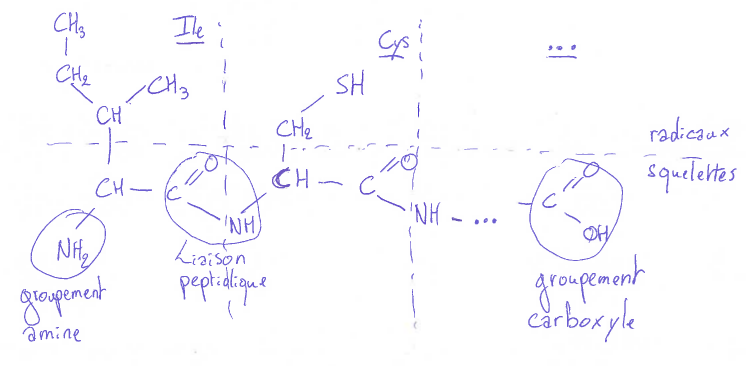
\includegraphics[width=400px]{Figures/bio/Intro/chaine_pep.png}
    \caption{\label{chaine_pep}Présentation d'une chaine peptidique.
    Chaque trait pointillé vertical sépare un acide aminé d'un autre et chaque trait horizontal sépare le squelette de la chaine latérale des acides aminés.}
  \end{center}
\end{figure}

\paragraph{}Une fois assemblée, une protéine se replie sur elle même et ce sont les caractéristiques structurelles et physico-chimiques qui en découlent qui donnent son activité.
Plus précisément, ce sont les propriétés des éléments en contact avec l'extérieur de la protéine (les atomes qui ne se retrouvent pas enfermé au milieu du repliement) qui déterminent l'activité de celle-ci.
Ces propriétés sont donc très dépendantes du repliement et des types de radicaux exposés.



\subsection{Généralités sur les peptides non ribosomiques}
\paragraph{}Les peptides non ribosomiques (Non Ribosomal Peptide (NRP)) sont des petits polymères synthétisés par certaines bactéries et certains champignons unicellulaires.
Tout comme les protéines classiques, les NRP sont des des molécules résultant d'assemblages de briques de base.
Cependant, comme le nom l'indique, la voie de synthèse d'un NRP est différente de celle des protéines.
Cette voie de synthèse comporte une étape supplémentaire.
Comme nous venons de le présenter, lors d'une création classique de protéine, l'ADN est transcrit en ARN qui lui même est traduit en protéine.
Ici, la protéine produite n'est pas le produit final mais une enzyme qui peut agir seule ou se grouper en complexes afin d'assembler
des NRP.
Ces complexes sont appelés des synthétases (Non Ribosomal Peptide Synthetase (NRPS)).
Là où les protéines classiques sont composées des 20 acides aminés standards, la synthèse non ribosomique permet
l'incorporation de plusieurs centaines de {\em monomères} (briques de bases) différents.


\begin{figure}[h!]
  \begin{center}
    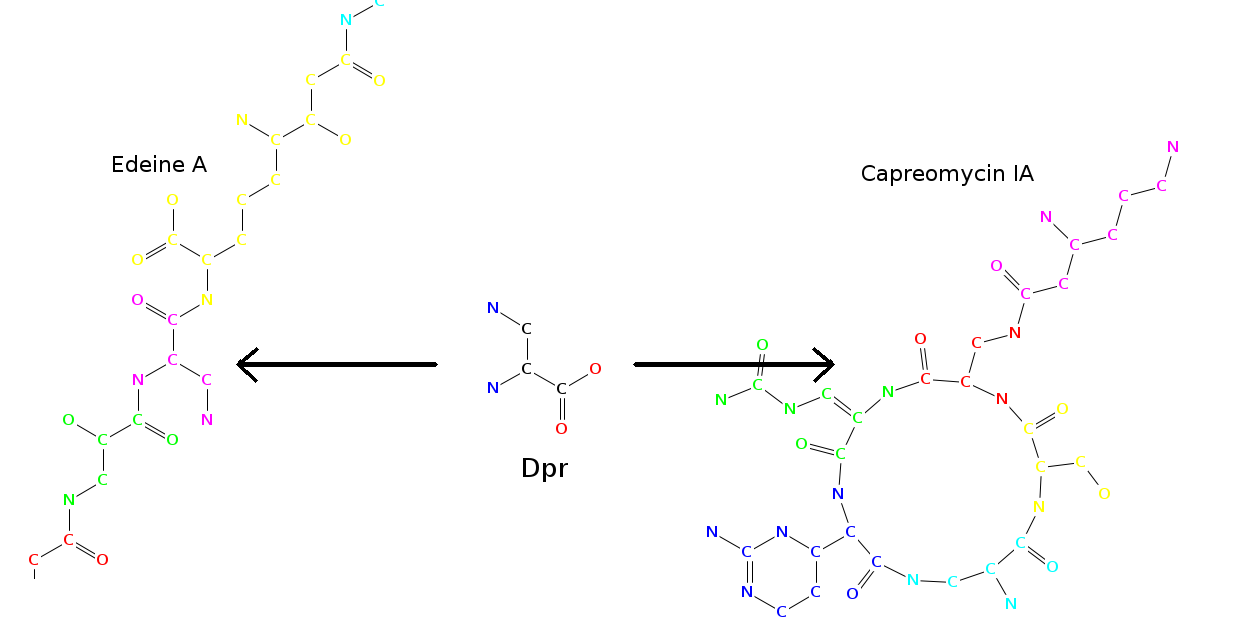
\includegraphics[width=480px]{Figures/bio/Intro/Dpr/2-3_liaisons.png}
    \caption{\label{DPR_incl}Deux exemples d'inclusion du monomère Dpr.
    Au sein de l'Edeine A, seules les deux liaisons classiques du squelette peptidique sont effectuées entre le Dpr et les autres monomères.
    Au sein de de la Capreomycin IA, une troisième liaison est effectuée par le Dpr depuis son groupement amine de la chaine latérale.}
  \end{center}
\end{figure}

\paragraph{}Les NRPS sont également plus souples dans la façon d'incorporer des monomères.
Certains monomères possèdent plus de deux groupements capables de se lier.
Ainsi sur l'exemple (Voir figure \ref{DPR_incl}), on peut constater que le monomère nommé Drp possède un groupement amine supplémentaire à celui déjà présent dans le squelette des acides aminés classiques.
Ce groupement en bout de chaine latérale permet au Drp de parfois se lier 3 fois et ainsi de casser la linéarité de la molécule assemblée.
Ce genre monomères, permet lorsqu'ils sont inclus, d'obtenir des structures à embranchements ou cycles.

\paragraph{TODO : Schéma exhaustif de NRPs}


\paragraph{}Les NRP présentent une grande diversité d'activités, souvent cruciales pour leurs producteurs.
Beaucoup de NRP recensés sont par exemple des antibiotiques.
La célèbre molécule de pénicilline est par exemple synthétisée à partir d'un précurseur NRP appelé ACV\cite{queener_molecular_1990}.
La diversité d'activités peut être expliquée par les grandes variations de structure et de composition par rapport aux protéines.
La possibilité d'effectuer des structures différentes contraint les repliements et la diversité de monomères permet la mise en contact avec l'extérieur, de structures moléculaires différentes.
L'efficacité des NRP produit peut quant à elle être expliqué par un effet de sélection.
La quantité d'énergie dépensée par la cellule pour produire un NRPS est énorme.
Si cette débauche d'énergie n'aboutissait sur rien, il y a fort à parier que la sélection naturelle aurait favorisé la suppression de ces fonctionnalités.


\subsection{Généralité sur les synthétases}

\paragraph{}Comme nous l'avons vu dans la courte introduction précédente, les synthétases permettant l'assemblage des NRP sont des protéines issues d'une synthèse classique.
Chaque NRPS est un complexe enzymatique extrêmement grand dont la taille est parfois à comparer à un ribosome (TODO : exemple taille en aa).
Cependant, contrairement à un ribosome, les NRPS sont spécialisés.
Un NRPS ne peut produire qu'un seul type de NRP.
Elles sont organisées en modules consécutifs qui permettent de capturer modifier et intégrer un monomère au NRP.
Chacun de ces modules peut à son tour être découpé en domaines fonctionnels.
Généralement un module est constitué de 3 domaines principaux et éventuellement de domaines optionnels.
Un module standard est d'abord composé d'un domaine de condensation (C) permettant la liaison du peptide déjà formé au monomère encours d'inclusion puis d'un module d'adénilation (A) permettant la capture du monomère à insérer et d'un module thiolation (T) effectuant la fixation du monomère capturé et le transfert du NRP depuis le domaine C précédent au domaine C suivant.
Il se peut que un ou plusieurs domaines permettant des modifications sur le monomère inclus, soient présents entre le domaine A et le domaine T.
Le premier module est également une exception à la règle du C-A-T car il ne possède normalement pas de domaine C (Car il n'y a rien à lier).

\begin{figure}[h!]
  \begin{center}
    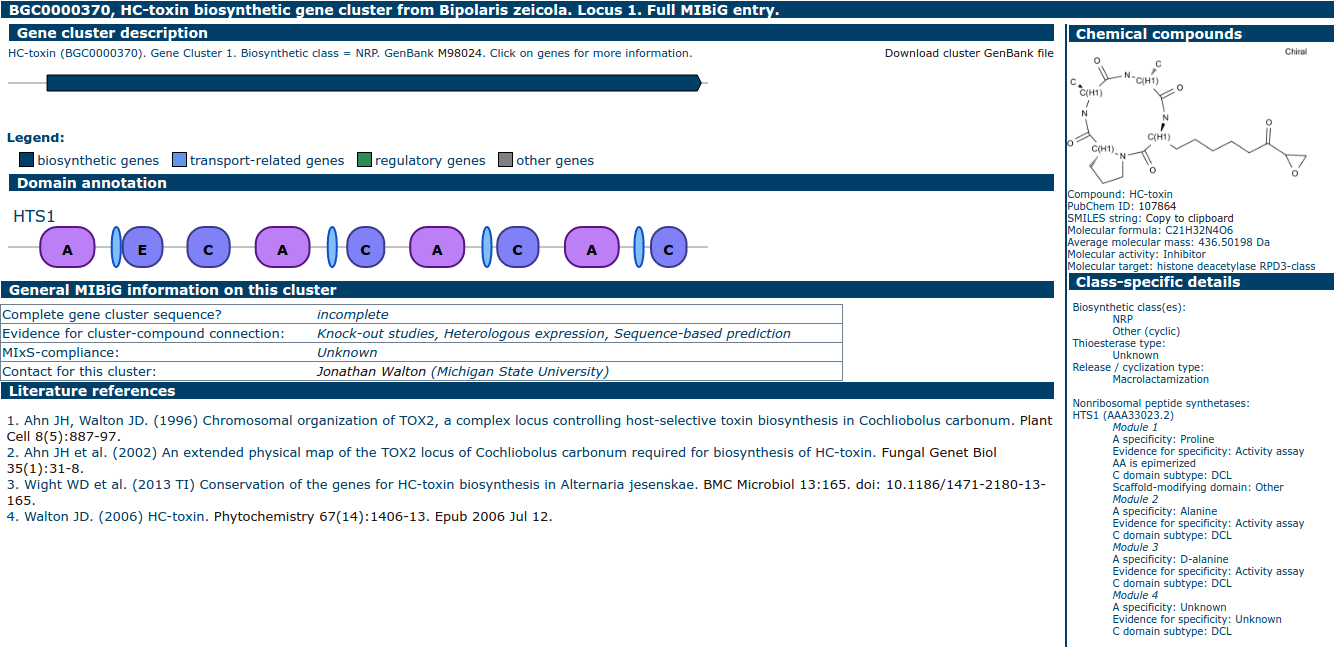
\includegraphics[width=480px]{Figures/bio/Intro/hc-toxin.png}
    \caption{\label{mibig_hc}Modules NRPS pour la création du peptide HC-Toxin.
    Image issue du site web MiBIG.}
  \end{center}
\end{figure}

\paragraph{}Prenons pour exemple le NRP appelé hc-toxin\cite{_mibig:_????}.
Le hc-toxin est un peptide non ribosomique composé de 4 monomères.
D'après la base de données MiBig couplée à celle du NCBI, la synthétase permettant sa création est composée de 5218 acides aminés.
Cette enzyme peut être séparée en 4 modules, chacun permettant l'inclusion d'un monomère.
Chacun des modules est également découpé en domaines.
Le découpage pour ce NRP est représenté sur la figure \ref{mibig_hc}.
Aux 4 modules correspondent 4 modules A, 4 modules T et 3 modules C.
On peut également voir un module d'épimérisation (modification de l'acide aminé inclus) présent en fin de premier module ainsi qu'un module C supplémentaire en fin d'enzyme permettant la cyclisation du peptide.

\subsection{Les domaines principaux}

\subsubsection{Le domaine d'Adénilation (domaine A)}

\paragraph{}C'est le domaine qui porte la spécificité du module dans lequel il se trouve.
La séquence d'acides aminés de ce domaine varie fortement afin de pouvoir capturer beaucoup de monomères différents.
Une fois le repliement de la synthétase effectué, les domaines A possèdent une cavité interne permettant la reconnaissance et l'accueil d'une molécule.
Ce sont les acides aminés de la synthétase en contact avec cette cavité qui vont permettre de "choisir" le monomère à capturer dans l'environnement.
La taille de la cavité ainsi que les propriétés physico-chimiques de ces acides aminés en contact permettent une affinité forte avec un unique monomère.
Il arrive parfois que le domaine ne soit pas spécifique à un seul monomère mais plutôt à un petit nombre de monomères très proches les uns des autres.
Cependant ce cas reste rare et dans la majorité des cas,  un NRPS ne permet la création que d'un seul NRP.

\paragraph{}En 1999, Stachelhaus et al. publient un article analysant la structure de nombreux domaines A\cite{stachelhaus_specificity-conferring_1999}.
Ils essayent d'aligner un grand nombre de domaines A pour en extraire les parties conservées et les parties spécifiques au monomère à capturer.
Il apparait que très peu d'acides aminés sont conservés d'un domaine A à l'autre mais que ceux-ci peuvent être utilisés comme marqueurs fixes.
Ces points conservés (et donc à priori très importants), permettent de servir de repères vers des acides aminés proches faisant partie de la poche d'accueil du monomère.
Les auteurs extraient un codage permettant de déterminer le monomère inclus à partir de 10 acides aminés présents dans la séquence d'un domaine A.
Depuis cet article, ce codage de référence est appelé code de Stachelhaus.


\subsubsection{Le domaine de Thiolation (domaine T)}
%citations : 
%• Biochemical characterization of peptidyl carrier protein (PCP), the thiolation domain of multifunctional peptide synthetases.
%• Portability of the thiolation domain in recombinant pyoverdine non-ribosomal peptide synthetases

\paragraph{}Le but du domaine T est d'assurer la logistique au sein du module dans lequel il est contenu\cite{stachelhaus_biochemical_1996,calcott_portability_2015}.
Ce domaine est également souvent appelé "Peptidyl Carrier domain".
Il est en charge de la récupération et du transfert du peptide en cours de formation.
Chaque domaine T possède un groupement 4’-phosphopantetheine incluant un "bras flexible" qui permet d'agripper et de déplacer les monomères.
Dans un premier temps, ce bras permet d'aller chercher le monomère capturé par le domaine A voisin et de le lier de manière covalente.
Dans un second temps, le monomère est mené au le site de condensation du début de module afin d'être inséré par le domaine C au début du NRP déjà formé.
Enfin, le bras se plie dans la direction du domaine de condensation suivant afin de lier le NRP au monomère suivant.
Durant cette étape, le peptide est libéré du domaine T courant pour être laissé à la charge du domaine T suivant.

\paragraph{Schéma du domaine T}

\subsubsection{Le domaine de Condensation (domaine C)}
%citations :
%• Peptide Bond Formation in Nonribosomal Peptide Biosynthesis, CATALYTIC ROLE OF THE CONDENSATION DOMAIN
%• http://bmcevolbiol.biomedcentral.com/articles/10.1186/1471-2148-7-78

\paragraph{}Le domaine C est par convention considéré comme le premier domaine de chaque module\cite{stachelhaus_peptide_1998}.
C'est un domaine qui permet de lier le morceau de peptide assemblé par les modules précédents avec le monomère capturé par le domaine A du module courant.
Bien que sa fonction principale reste toujours la même, il existe plusieurs variants\cite{rausch_phylogenetic_2007} de ce domaine que nous allons décrire par la suite.

\paragraph{Les domaine LCL et DCL}
Les acides aminés capturés par les domaines A existent dans deux configuration différentes dites configurations L et D.
Il existe deux domaines C différents pour lier ces molécules.
Le plus standard, permet la liaison de deux monomères de type L. Le domaine est alors appelé domaine LCL.
Le second permet de lier un monomère D à un L, il est alors appelé domaine DCL.
Ces domaines sont juste deux spécialisations du modèle décrit ci-dessus.

\paragraph{Les domaines C starter (Cs) et C terminal (Ct)}
Comme leur noms l'indiquent ces domaines sont en bout de protéines.
Il ne sont donc pas entouré de deux modules différents mais sont inclus respectivement dans le premier et dernier modules.
Il ne peuvent donc faire la liaison entre deux monomères fixés sur deux bras de domaines T.

\paragraph{}Le domaine Cs permet de directement capturer et lier un monomère de l'environnement afin de débuter le peptide.
Cela permet d'inclure par exemple des acides gras qui n'aurait pas de domaines A spécifiques.
Ces modules capturent toujours le même type de monomère mais on ne sait actuellement pas exactement comment cette spécificité est encodée dans l'enzyme.

\paragraph{}Le rôle du domaine Ct est lui un peu plus flou.
Dans certains peptides ce domaine permet de faire une liaison entre le dernier monomère et un monomère déjà inclus, créant ainsi un cycle.
Dans d'autres il lie le dernier monomère avec un monomère de l'environnement.
Comme pour le Cs, la spécificité n'est pas encore expliquée.
Il est également possible que les deux comportements soient en fait issus de deux sous catégories de Ct mais rien n'a encore été prouvé.

\paragraph{Le domaine Cy}
Cette dernière variation du module C standard permet de lier deux monomères voisins en effectuant deux liaisons.
Cette liaison est toujours effectuée par un monomère possédant un atome de soufre près d'un groupement amine.

\begin{figure}[h!]
  \begin{center}
    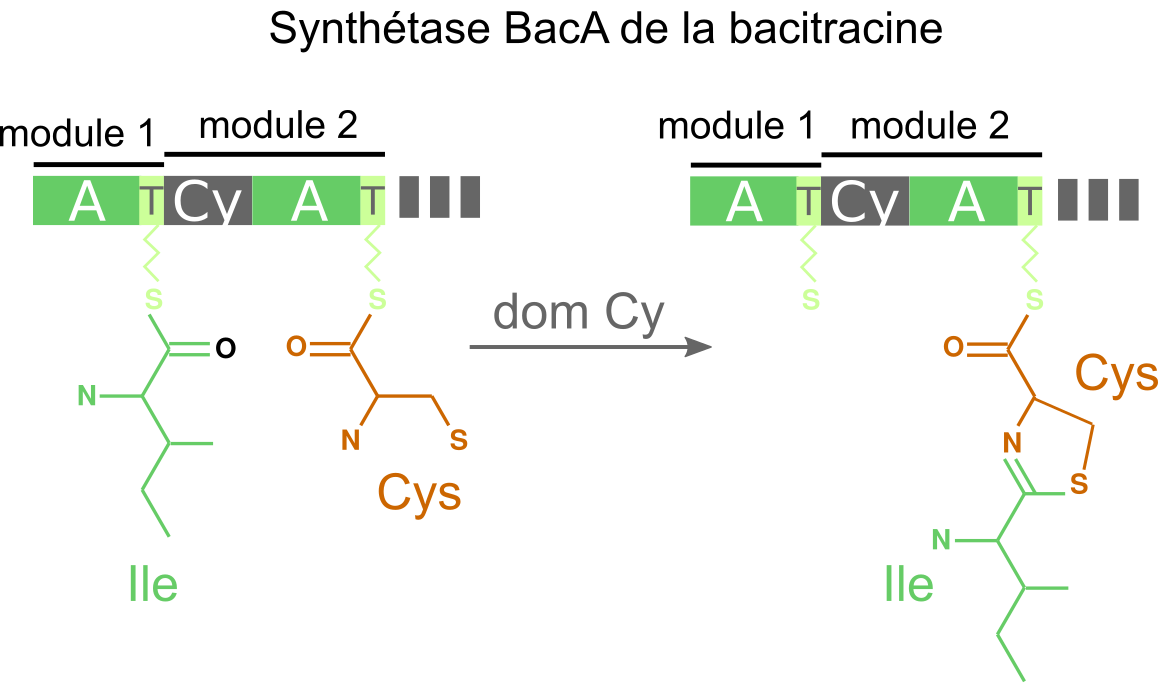
\includegraphics[width=300px]{Figures/bio/Intro/domainCy_bacitracine.png}
    \caption{\label{domaine_Cy}Cyclisation entre deux monomères par un domaine Cy}
  \end{center}
\end{figure}


\subsubsection{Le domaine de Thioestérase}

\paragraph{}Contrairement aux 3 autres domaines principaux, celui-ci ne fait partie d'aucun module.
C'est un module de terminaison qui permet le décrochage du peptide complètement formé.
Ce module de séparation n'est pas toujours présent et sa fonction est parfois exprimée par d'autres modules comme le Ct.


\subsection{Les domaines de transformation monomérique}

\paragraph{}Nous allons à présent parler de quelques modules optionnels permettant de modifier un monomère capturé par un domaine A.
Ces transformations permettent aux organismes d'obtenir des configurations monomériques peu fréquentes dans leur environnement.


\paragraph{La fonction d'épimérisation (domaines E et C/E)}

Lors de la description des domaines LCL et DCL, nous avons rapidement évoqué la possibilité pour une molécule d'être dans deux configurations différentes tout en possédant pour autant la même composition et structure atomique.
Ces deux configuration sont en fait des images miroirs l'une de l'autre.
On appel ces deux configurations Leavus (L) et Dexter (D).

\begin{figure}[h!]
  \begin{center}
    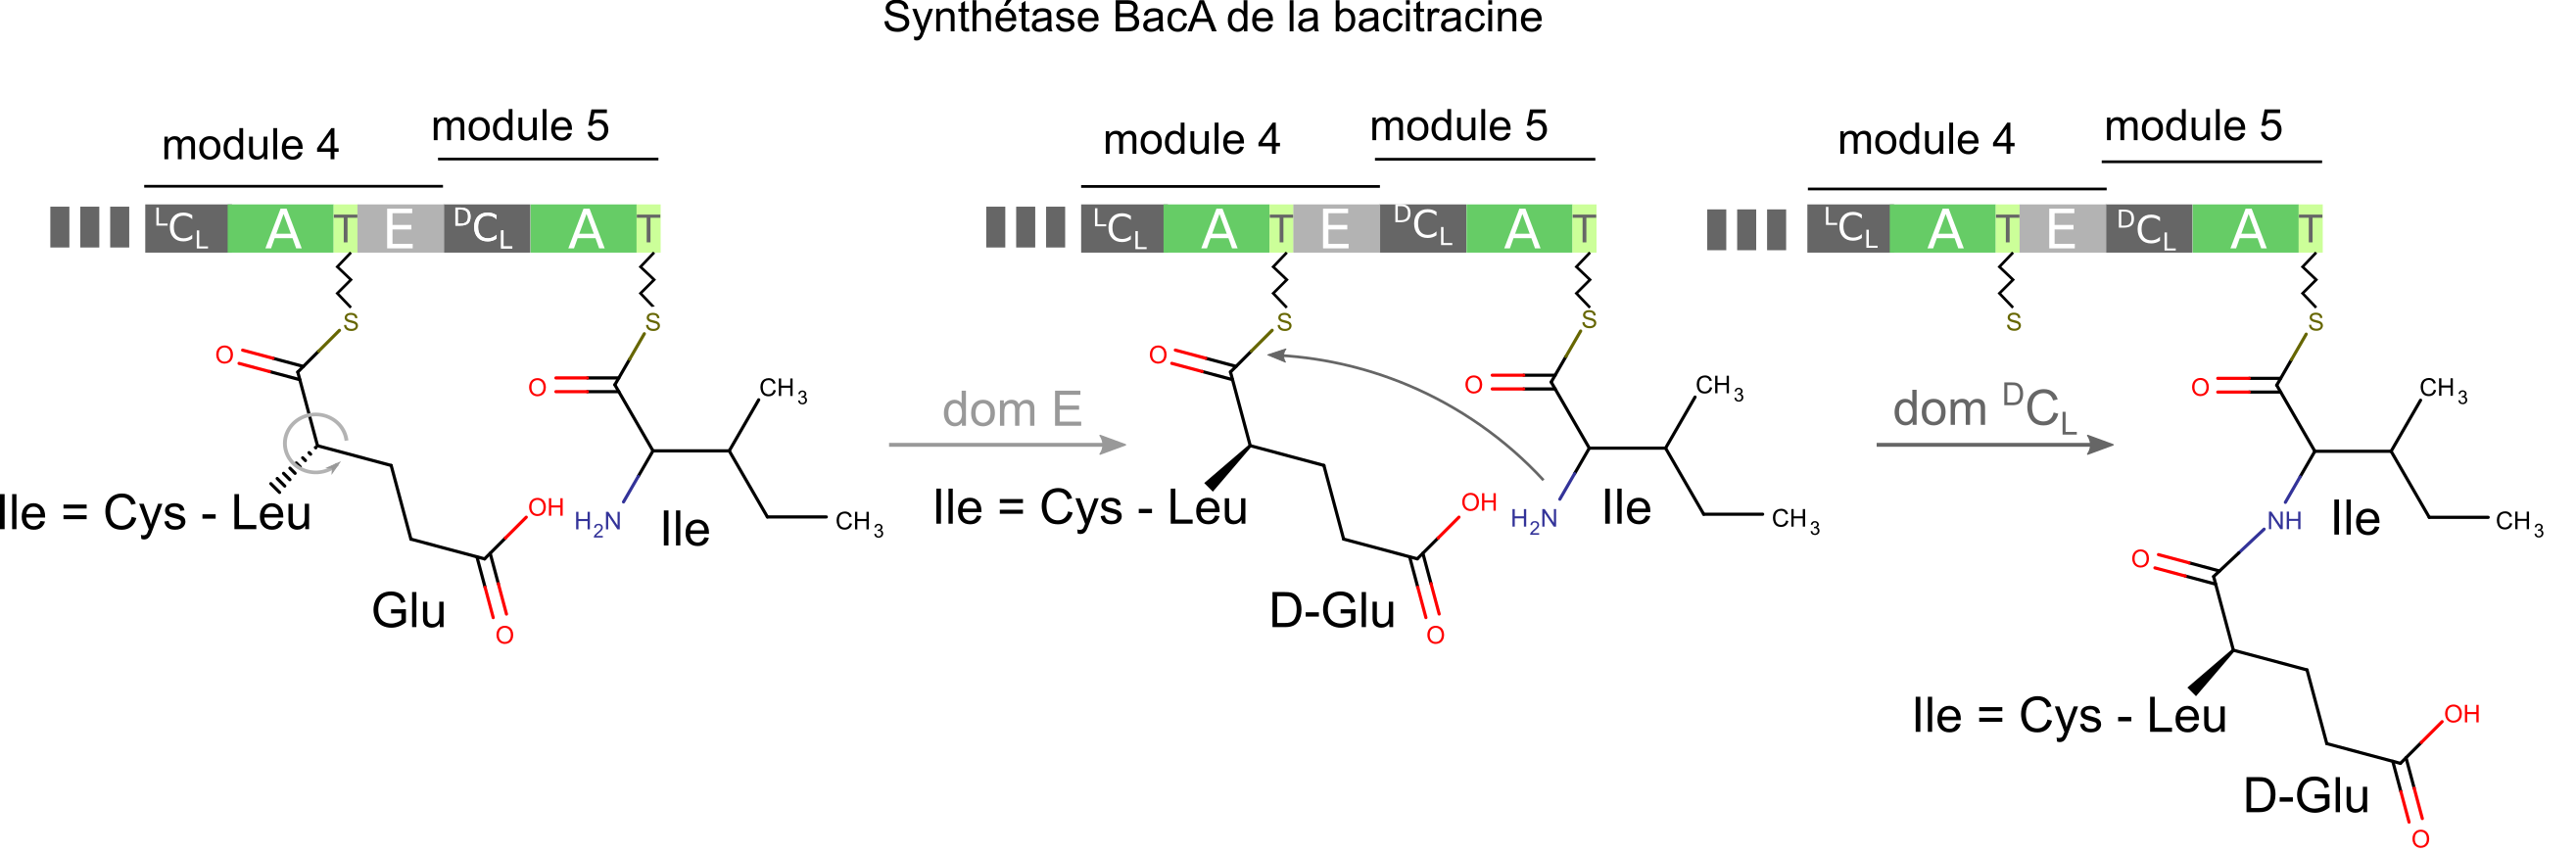
\includegraphics[width=400px]{Figures/bio/Intro/domaineE-bacitracine.png}
    \caption{\label{domaine_E}Épimérisation d'un monomère par un domaine E}
  \end{center}
\end{figure}

\paragraph{}Alors que la majorité de la vie est gauchère (ne contient que des acides aminés L), les NRPS permettent l'inclusion de monomères de forme D en capturant un monomère L puis en le transformant.
Les domaines responsables de ces transformation sont appelés domaines d'épimérisation.
Une fois le monomère L lié au reste du peptide par le domaine C, il est emmené auprès du domaine E afin de changer son orientation.
Le fait que cette transformation soit postérieure à la fixation sur le reste du peptide explique l'absence de domaines DCD (Les monomères de droite seront toujours présentés au domaine C avant transformation).
Il arrive parfois que cette transformation du monomère ne soit pas portée par un domaine E mais directement incluse dans le domaine C précédent.
Ce domaine est alors appelé domaine C/E et assure les deux fonctionnalités.


\paragraph{domaine de N-méthylation (NM)}

De la même manière que le domaine E, le domaine NM agit à la suite de la liaison du monomère actuel au morceau de peptide précédemment assemblé.
Ce domaine permet l'ajout d'un méthyle (CH3) sur le groupement amine du monomère courant.

\begin{figure}[h!]
  \begin{center}
    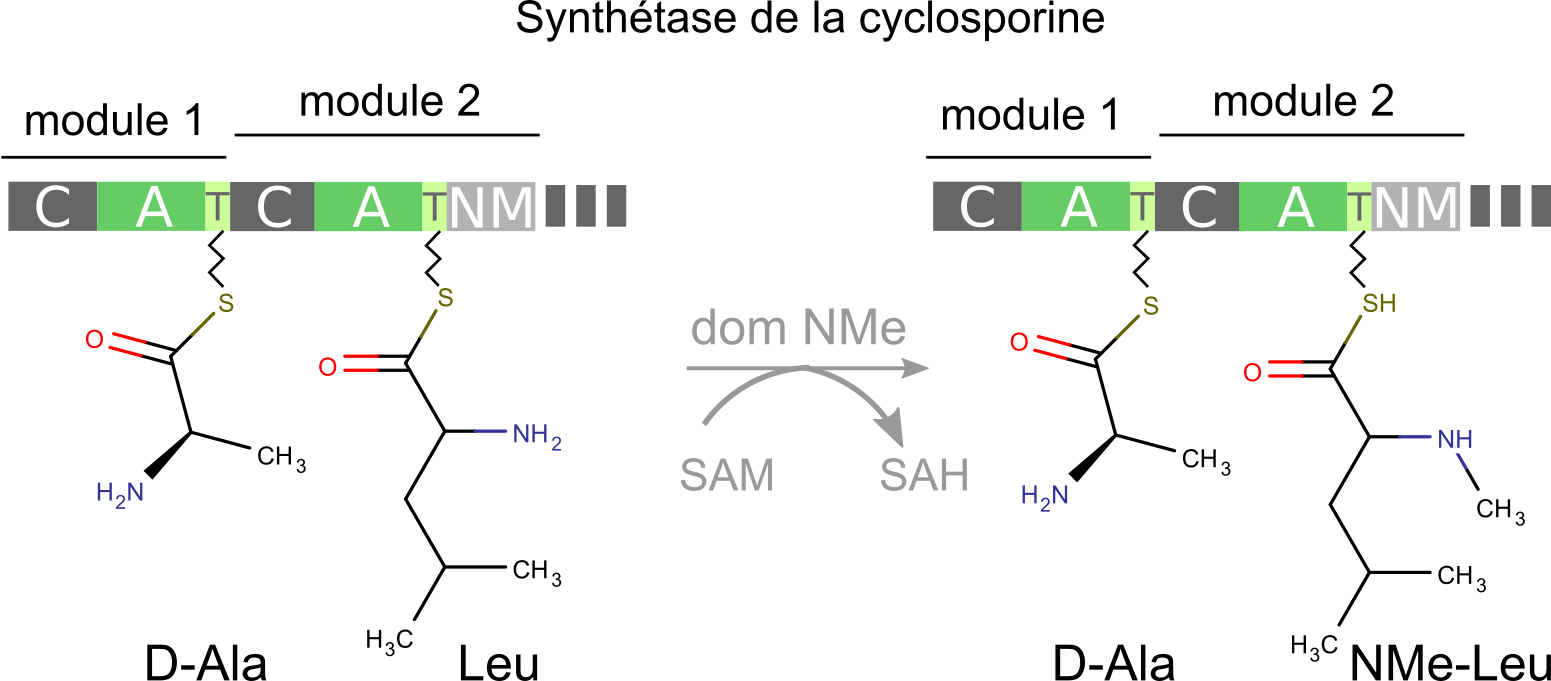
\includegraphics[width=300px]{Figures/bio/Intro/domaineNMe-cyclosporine.png}
    \caption{\label{domaine_NMe}Méthylation d'un monomère par un domaine NM}
  \end{center}
\end{figure}

\paragraph{domaine de formylation}
% http://archiv.ub.uni-marburg.de/diss/z2008/0068/pdf/dgs.pdf

Ce domaine n'existe à priori que pour les modules d'initiation.
Il permet la formylation (ajout d'un groupe C(=O)H) sur le groupement amine du premier monomère\cite{schonafinger_amide_2007}.

\begin{figure}[h!]
  \begin{center}
    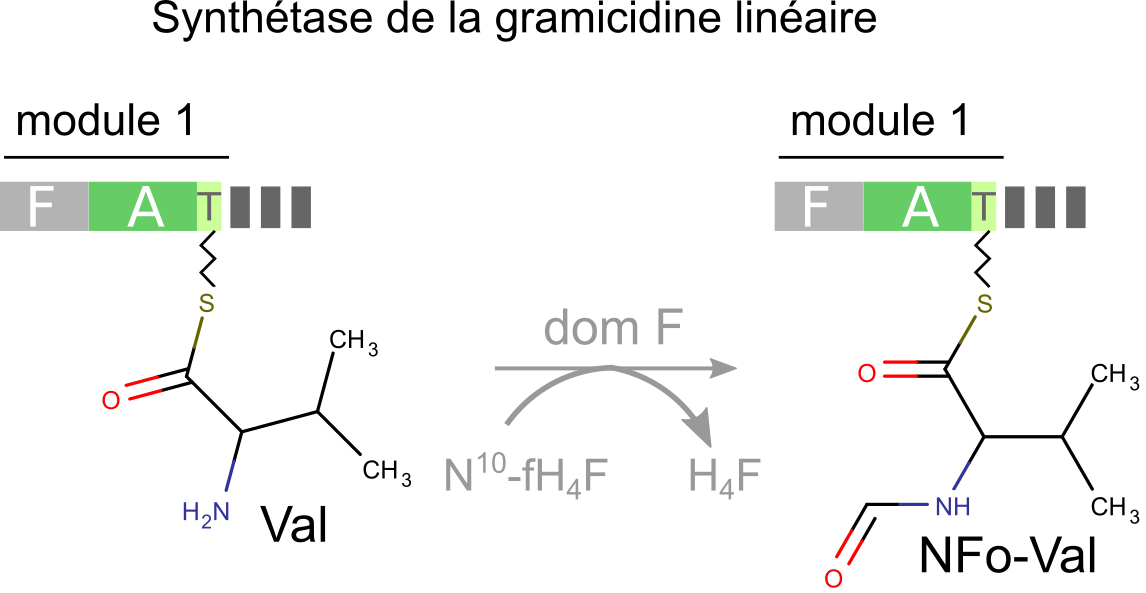
\includegraphics[width=300px]{Figures/bio/Intro/domaineF-gramicidine.png}
    \caption{\label{domaine_F}Formilation d'un monomère par un domaine F}
  \end{center}
\end{figure}


\subsection{Incorporations extra-NRPS}

\paragraph{}Depuis le début de cette partie, nous parlons de synthèse non ribosomique.
Cependant, il arrive que le produit délivré par la synthétase et le produit final trouvé dans l'environnement de la cellule ne soient pas les mêmes.
Lorsque cette différence est constatée, c'est que le peptide a subit une transformation entre la fin de sa synthèse non ribosomique et le moment où il est effectivement en activité.
Toutes les modifications ponctuelles sont effectuées par des enzymes de décoration.
Parfois il arrive que ce soit une partie complète de la molécule qui ne soit pas NRP.
Il existe des molécules très proches des NRP appelés polyketides qui peuvent venir s'hybrider avec des NRP.
Dans cette partie nous allons aborder ces deux types de modification d'un NRP.


\subsubsection{Les enzymes de décoration}

\paragraph{}Les clusters de gènes de NRPS ne sont pas uniquement constitués des gènes d'enzymes NRPS.
Tout un tas de gènes accompagnateurs sont présent au même endroit.
Parmi ceux-ci, certains gènes servent à modifier les NRP après leur production.
La vancomycine est un très bon exemple de modifications enzymatiques post-synthèse.

\begin{figure}[h!]
  \begin{center}
    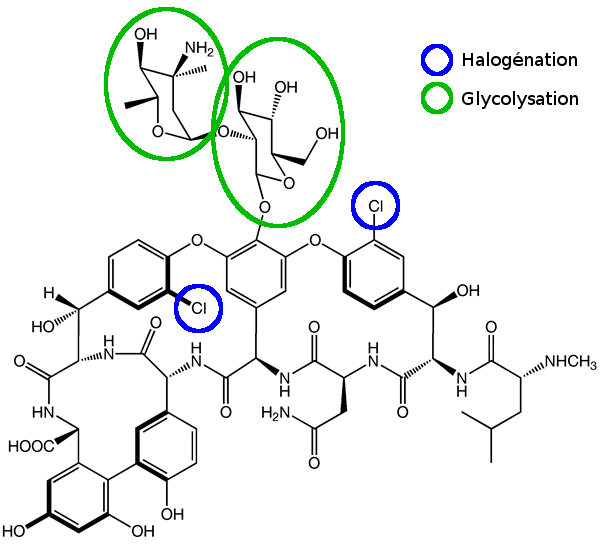
\includegraphics[width=300px]{Figures/bio/Intro/vanco.png}
    \caption{\label{vanco}Modifications post-synthèse NRP pour la vancomycine}
  \end{center}
\end{figure}

\paragraph{}Sur la figure \ref{vanco}, les deux structures entourées en vert se démarquent par rapport au reste de la molécule.
Ce sont deux sucres qui ont été ajoutés après la synthèse (un vancosamine et un D-glucose).
Les sucres sont des monomères qui ne peuvent pas être capturés par des domaines A.
Ce sont des gènes extérieurs à la NRPS qui sont dédiés à leur capture, transformation et liaison avec la NRP.
Ce phénomène d'ajout de sucre est appelé glycosylation.
Comme le suggère \cite{van_wageningen_sequencing_1998} trois enzymes sont en action pour l'incorporation de la vancosamine.
La vancosamine n'étant pas naturellement présent dans l'environement de l'organisme producteur, l'une des enzymes est dédiée à la création de ce sucre à partir du NDP-4-keto-6-deoxyglucose.

\paragraph{}La vancomycine possède également deux atomes de Clore.
Ces deux atomes sont inhabituels pour des NRP et ne sont pas initialement présent au sein de leur monomères de rattachement.
Il n'existe pas non plus de domaine NRPS capable d'inclure ce genre d'atomes.
Van Wageningen dans l'article précédemment cité montre également que deux enzymes issues du cluster de gène de la NRPS, sont responsables de ces incorporations.
Ce type d'enzyme est appelé enzyme d'halogénation car elle est capable d'inclure un atome halogène (Fluore, Clore, Brome, Iode, Astate)

\paragraph{}Pour résumer, les enzymes de décoration post-synthèse sont capable d'effectuer 3 tâches que nous avons découvert sur l'exemple de la vancomycine :
\begin{itemize}
  \item La synthèse de monomères en modifiant des composants de l'environnement (création de vancosamine)
  \item La création de liaison entre monomères de l'environnement et NRP (Les sucres de la vancomycine)
  \item La modification de morceaux de monomères déjà inclus dans le NRP (halogénation par exemple)
\end{itemize}

Toutes ces enzymes permettent à nouveau d'augmenter la combinatoire des molécules potentiellement créées.



\subsubsection{Les PKS}
% TODO : Reférences

\paragraph{}Les PKS (Polyketyde Synthetase) sont tout comme les NRPS des enzymes modulaires permettant de synthétiser des polymère complexes par une voie non ribosomique.
Cependant, contrairement aux NRPS, les PKS n'incorporent pas de monomères directement formés mais construisent les PK par ajouts successifs de quelques atomes.
De la même manière que les domaines A des NRPS capturent des monomères spécifiques, certains domaines PKS sont spécialisés pour effectuer des réactions permettant l'ajout de quelques atomes au PK en création.
Tout comme les NRP, les PK sont des molécules très coûteuses à produire mais très utiles pour les organismes qui les produisent.
Sur la figure \ref{pks} nous montrons le processus de synthèse d'une PK.

\begin{figure}
  \begin{center}
    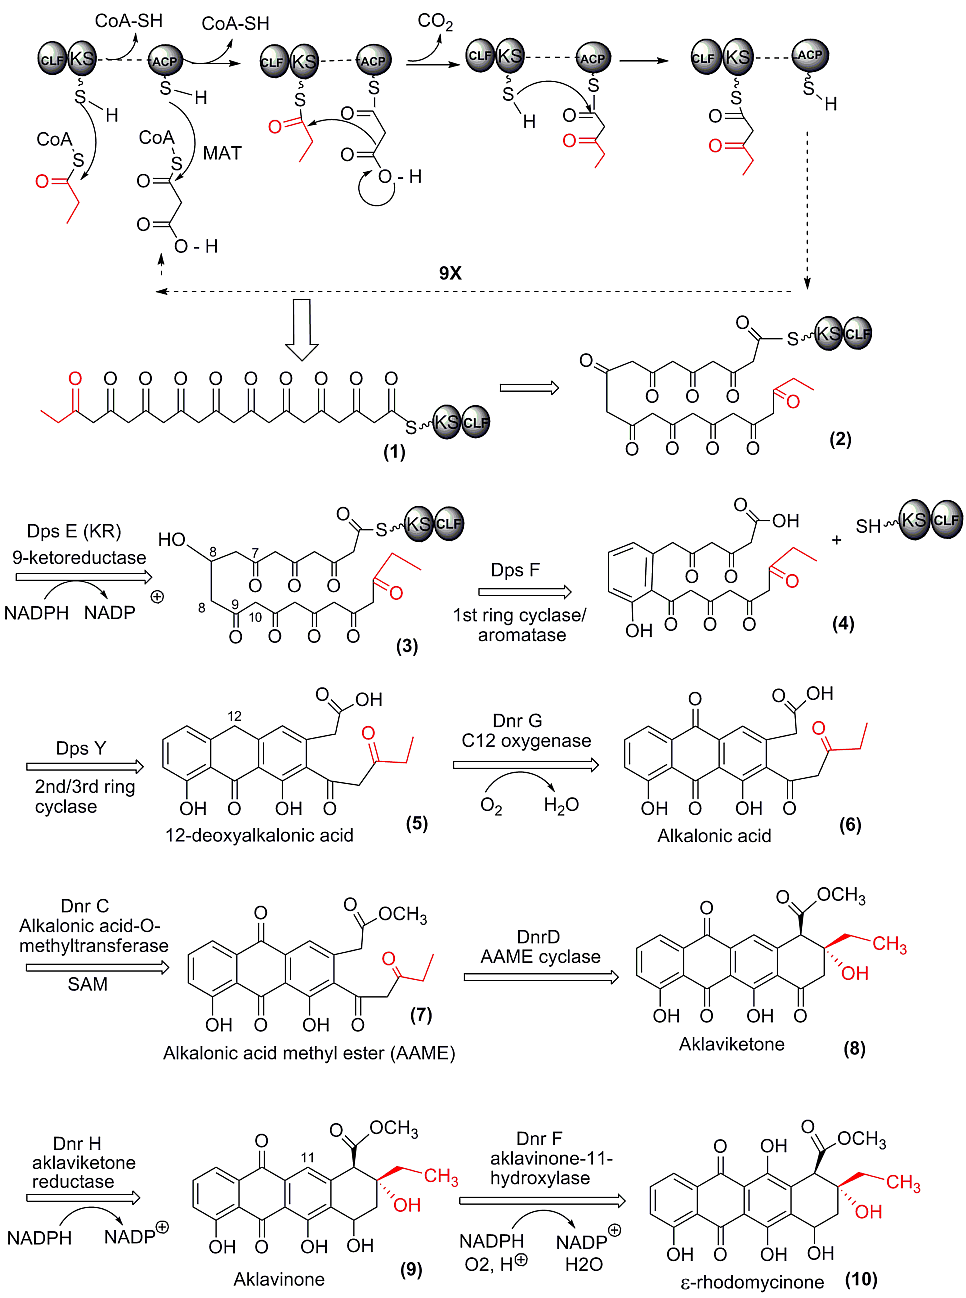
\includegraphics[width=400px]{Figures/bio/Intro/PKS.png}
    \caption{\label{pks}Synthèse d'une epsilon-rhodomycinone
    Comme pour les NRPS, les PKS sont constitués de modules fonctionnels.
    Sur cet exemple on peut voir que certains modules sont utilisés plusieurs fois itérativement.
    La longue chaine carbonée de la première étape est créée par une répétition successive de 9 fois le même module.
    Tout comme les NRP, les PK peuvent être modifiés après libération par le PKS (étapes 5 à 10 ici).
    Source de l'image : en.wikipedia.org/wiki/Polyketide\_synthase}
  \end{center}
\end{figure}

\paragraph{}Les PKS et NRPS ont des origines communes dans l'évolution et il est logique de les retrouver au mêmes endroits du génome.
Plusieurs NRP sont hybride avec des PK, le cluster de gènes est alors composé de gènes NRPS et PKS.
Il existe alors deux moyens de créer ces hybrides.
Soit la PK est créé séparément du NRP et les deux sont liés post-synthèse par des enzymes similaires aux enzymes décoratrices décrites précédemment.
Soit la PKS et la NRPS sont produit simultanément et s'assemblent pour former un gros complexe enzymatique hybride.
Le NRP-PK est alors directement formé pendant la synthèse en faisant passer le polymère en formation de module en module (qu'ils soient NRPS ou PKS).
A nouveau, cette hybridation avec d'autres types de polymères permet d'augmenter la quantité de conformations de peptides possibles.









\section{Les outils bioinformatiques pour l'annotation et l'analyse des NRP/NRPS}

\paragraph{}Après avoir présenté les NRP ainsi que leur voies de synthèse, nous allons nous attarder sur les outils bio-informatiques qui s'y intéressent.
Les outils que nous allons présenter ici se focalisent soit sur les NRPS soit sur les NRP, c'est pourquoi la présentation séparera distinctement ces deux types d'outils.
Pour chacune de ces catégorie, nous allons également distinguer deux sous catégories.
La première portera sur les outils permettant l'annotation des données.
Pour les NRPS l'annotation correspondra à la phase de recherche de gènes NRPS dans le génome ainsi qu'à l'identification des différentes briques contenues dans ces gènes (entre autre les modules).
Pour les NRP l'annotation correspondra à la phase d'identification et de décomposition des structures monomériques présentes dans des molécules.
La seconde sous-catégorie présentera les moyens d'archivage et de mise à disposition des informations récoltées par les outils d'annotation.
Cette partie rassemblera les différentes bases de données, dédiées ou non et contenant une ou plusieurs informations à propos des NRPS ou NRP.

\subsection{Les outils d'annotation de NRPS}

\paragraph{}Dans cette partie, nous allons nous attarder sur les outils bioinformatiques permettant la découverte et l'annotation de NRPS depuis le génome.
Cette recherche pourra être effectuée par étapes successives en commençant par la détection des clusters de gènes, en poursuivant par l'annotation des domaines des NRP et en finissant par les détections spécifiques aux types de clusters.

\subsubsection{Détection de clusters de gènes}

\paragraph{}L'information des clusters de gènes est très importante pour comprendre les formes finales de NRP.
La détection des clusters nous permet d'identifier l'ensemble des gènes impliqués dans la synthèse d'un NRP et pas uniquement ceux impliqués dans la création d'un NRPS.
Avoir accès à l'ensemble des gènes d'un cluster nous permet par exemple de détecter les transformations post-synthèse qui peuvent modifier un NRP.

\paragraph{}Il existe de nombreuses techniques permettant la recherche de clusters de gènes.
Certains outils génériques comme CLUSEAN\cite{weber_clusean:_2009} qui permettent de détecter des clusters de gène quels qu'ils soient.
L'inconvénient fort pour l'application aux NRPS, il est nécessaire de passer un second logiciel pour vérifier que le cluster est bien NRPS.
Il existe également des techniques spécialisées pour détecter directement des clusters de gène de métabolites secondaires.
Par exemple, le logiciel CASSIS\cite{wolf_cassis_2016} exploite des propriétés de régions promotrices pour découvrir et classifier ces clusters.

\paragraph{}De nombreux autres logiciels encore plus spécialisés existent.
Il est possible de découvrir des clusters de métabolites secondaires chez des bactéries\cite{cruz-morales_recapitulation_2015}, des champignons\cite{khaldi_smurf:_2010} ou encore plus précisément chez des champignons filamenteux\cite{andersen_accurate_2013,umemura_motif-independent_2015}.
Tout ces outils pour dire que quel que soit le sous domaine des NRP étudié, nous pouvons toujours trouver un outil spécialisé dans la recherche de leurs clusters de gènes.



\subsubsection{Détection et identification de domaines NRPS}

\paragraph{}La détection et l'identification des gènes codant pour les domaines est le coeur de l'annotaion des NRPS.
Nous allons ici présenter des méthodes qui permettent à la fois d'identifier les différents types de domaines (A, C, T, ...) ainsi que des méthodes permettant d'inférer les spécificités de ces domaines.

% Chapter 8 Methods for In Silico Prediction of Microbial Polyketide and Nonribosomal Peptide Biosynthetic Pathways from DNA Sequence Data
\paragraph{La recherche "manuelle"/automatique}
Il est possible de rechercher des domaines NRPS quasi-manuellement\cite{bachmann_chapter_2009}.
Pour cela, il faut constituer une petite base données de domaines NRPS très généralistes puis les rechercher dans le génome cible à l'aide d'algorithmes comme BLAST.
En analysant ensuite manuellement les alignements obtenus, il est possible de détecter certains domaines qui auraient été éliminés par des algorithmes automatiques.
Cette méthode reste dérisoire au regard de la quantité d'informations à gérer.
Elle n'est utilisée que dans des cas très particuliers où l'on suppose fortement la découverte de nouveaux éléments.
Cette technique peut également être utilisée automatiquement.
Après avoir les résultats des différents BLAST lancés, il est possible de mettre un seuil de ressemblance et d'annoter tous les domaines trouvés par le nom du domaine de référence le plus proche.

%· Specificity prediction of adenylation domains in nonribosomal peptide synthetases (NRPS) using transductive support vector machines (TSVMs)
%· NRPSpredictor2—a web server for predicting NRPS adenylation domain specificity
\paragraph{NRPS predictor}
NRPS prédictor\cite{rottig_nrpspredictor2web_2011,rausch_specificity_2005} est un outil de prédiction des substrats capturés par les domaines A.
Il analyse une séquence trouvée par un algorithme de détection de module A et prédit sa spécificité.
Cet outil est basé sur la recherche par Machines à Vecteurs de Support (Support Vector Machine (SVM)).
L'idée est de se baser sur les données de domaines A déjà annotés afin de créer des séquences (vecteurs) caractéristiques des domaines.
L'outil permet de prédire les domaines A avec différents niveaux de granularité, ce qui permet d'avoir de l'information même lorsque le module A précis n'est pas détecté.
Le niveau le plus fin permet la détection exacte du monomère mais il est également possible de prédire les spécificités par "groupements" de monomère.
Par exemple, l'outil essayera de prédire si le monomère inclus est polaire, hydrophobique, aliphatique...
Chacun de ces critères ayant son propre profil SVM.
Cet outil est bien plus performant que le simple code de Stachelhaus et obtient une F-mesure de 80\% pour la prédiction la plus fine et 95\% pour les plus gros groupements de monomères.


% The Natural Product Domain Seeker NaPDoS: A Phylogeny Based Bioinformatic Tool to Classify Secondary Metabolite Gene Diversity
\paragraph{NaPDoS et l'identification des domaines C}
NaPDoS\cite{ziemert_natural_2012} est un logiciel issu d'un travail sur la phylogénie des domaines C NRPS.
Les auteurs ont créé une base de domaines C de NRPS déjà connus.
À partir de cette base, ils ont alignés tous les domaines les uns contre les autres et construit une phylogénie.
Cette phylogénie à permis aux auteurs de diviser les domaines C en plusieurs groupes et ainsi de créer la première classification de ces domaines.
Ces groupes ont été transformés en différentes HMM représentatives utilisées pour la classification des domaines au travers du serveur web de l'application.


% Chapter 8 Methods for In Silico Prediction of Microbial Polyketide and Nonribosomal Peptide Biosynthetic Pathways from DNA Sequence Data
\paragraph{2metDB - PKS/NRPS web server}
Ces deux logiciels sont deux implémentations de la même technique de détection des domaines NRPS et PKS\cite{bachmann_chapter_2009}.
La différence entre les deux est que 2metDB est un outil standalone alors que PKS/NRPS web server est une version en ligne.
Les auteurs font le constat qu'un domaine NRPS ou PKS possède des zones très variables en composition ainsi que des zones très conservées.
Ce sont ces zones conservées qui ont permis de déterminer des coordonnées fixes entre domaines A et ansi de créer le code de Stachelhaus.
Il existe des zones conservées au sein de tous les domaines.
Les auteurs des logiciels ont tiré partie de ces zones en créant des HMM pour représenter des archétypes pour chacun des types de domaine.
L'utilisation de HMM en faible nombre permet à ces logiciels d'être extrêmement rapide pour les recherches.


%· antiSMASH: rapid identification, annotation and analysis of secondary metabolite biosynthesis gene clusters in bacterial and fungal genome sequences
%· antiSMASH 3.0-a comprehensive resource for the genome mining of biosynthetic gene clusters
\paragraph{Antismash, le pipline pour l'identification de métabolites secondaires}
Antismash est sans doute le logiciel qui est venu révolutionner ces dernières années la prédiction de métabolites secondaire depuis l'ADN.
Le logiciel est un pipline incluant de nombreux outils dont ceux que nous avons décrit précédemment.
Les outils sont lancés les uns après les autres en analysant les séquences avec une granularité de plus en plus fine.
A un instant donné, en fonction des spécificité des génomes et des annotations réalisées précédemment sur un génome en cours d'analyse, Antismash va choisir les logiciels à lancer pour raffiner les prédictions.
Par exemple, en lançant une analyse sur un génome bactérien, Antismash va commencer par rechercher les clusters de gène avec CLUSEAN, puis identifier parmi les clusters détectés, ceux qui permettent la production de métabolites secondaires pour finir par lancer les outils spécifiques à chaque métabolite comme NRPS predictor et NAPDOS sur les clusters NRPS.

%Streptomyces coelicolor
\begin{figure}
  \begin{center}
    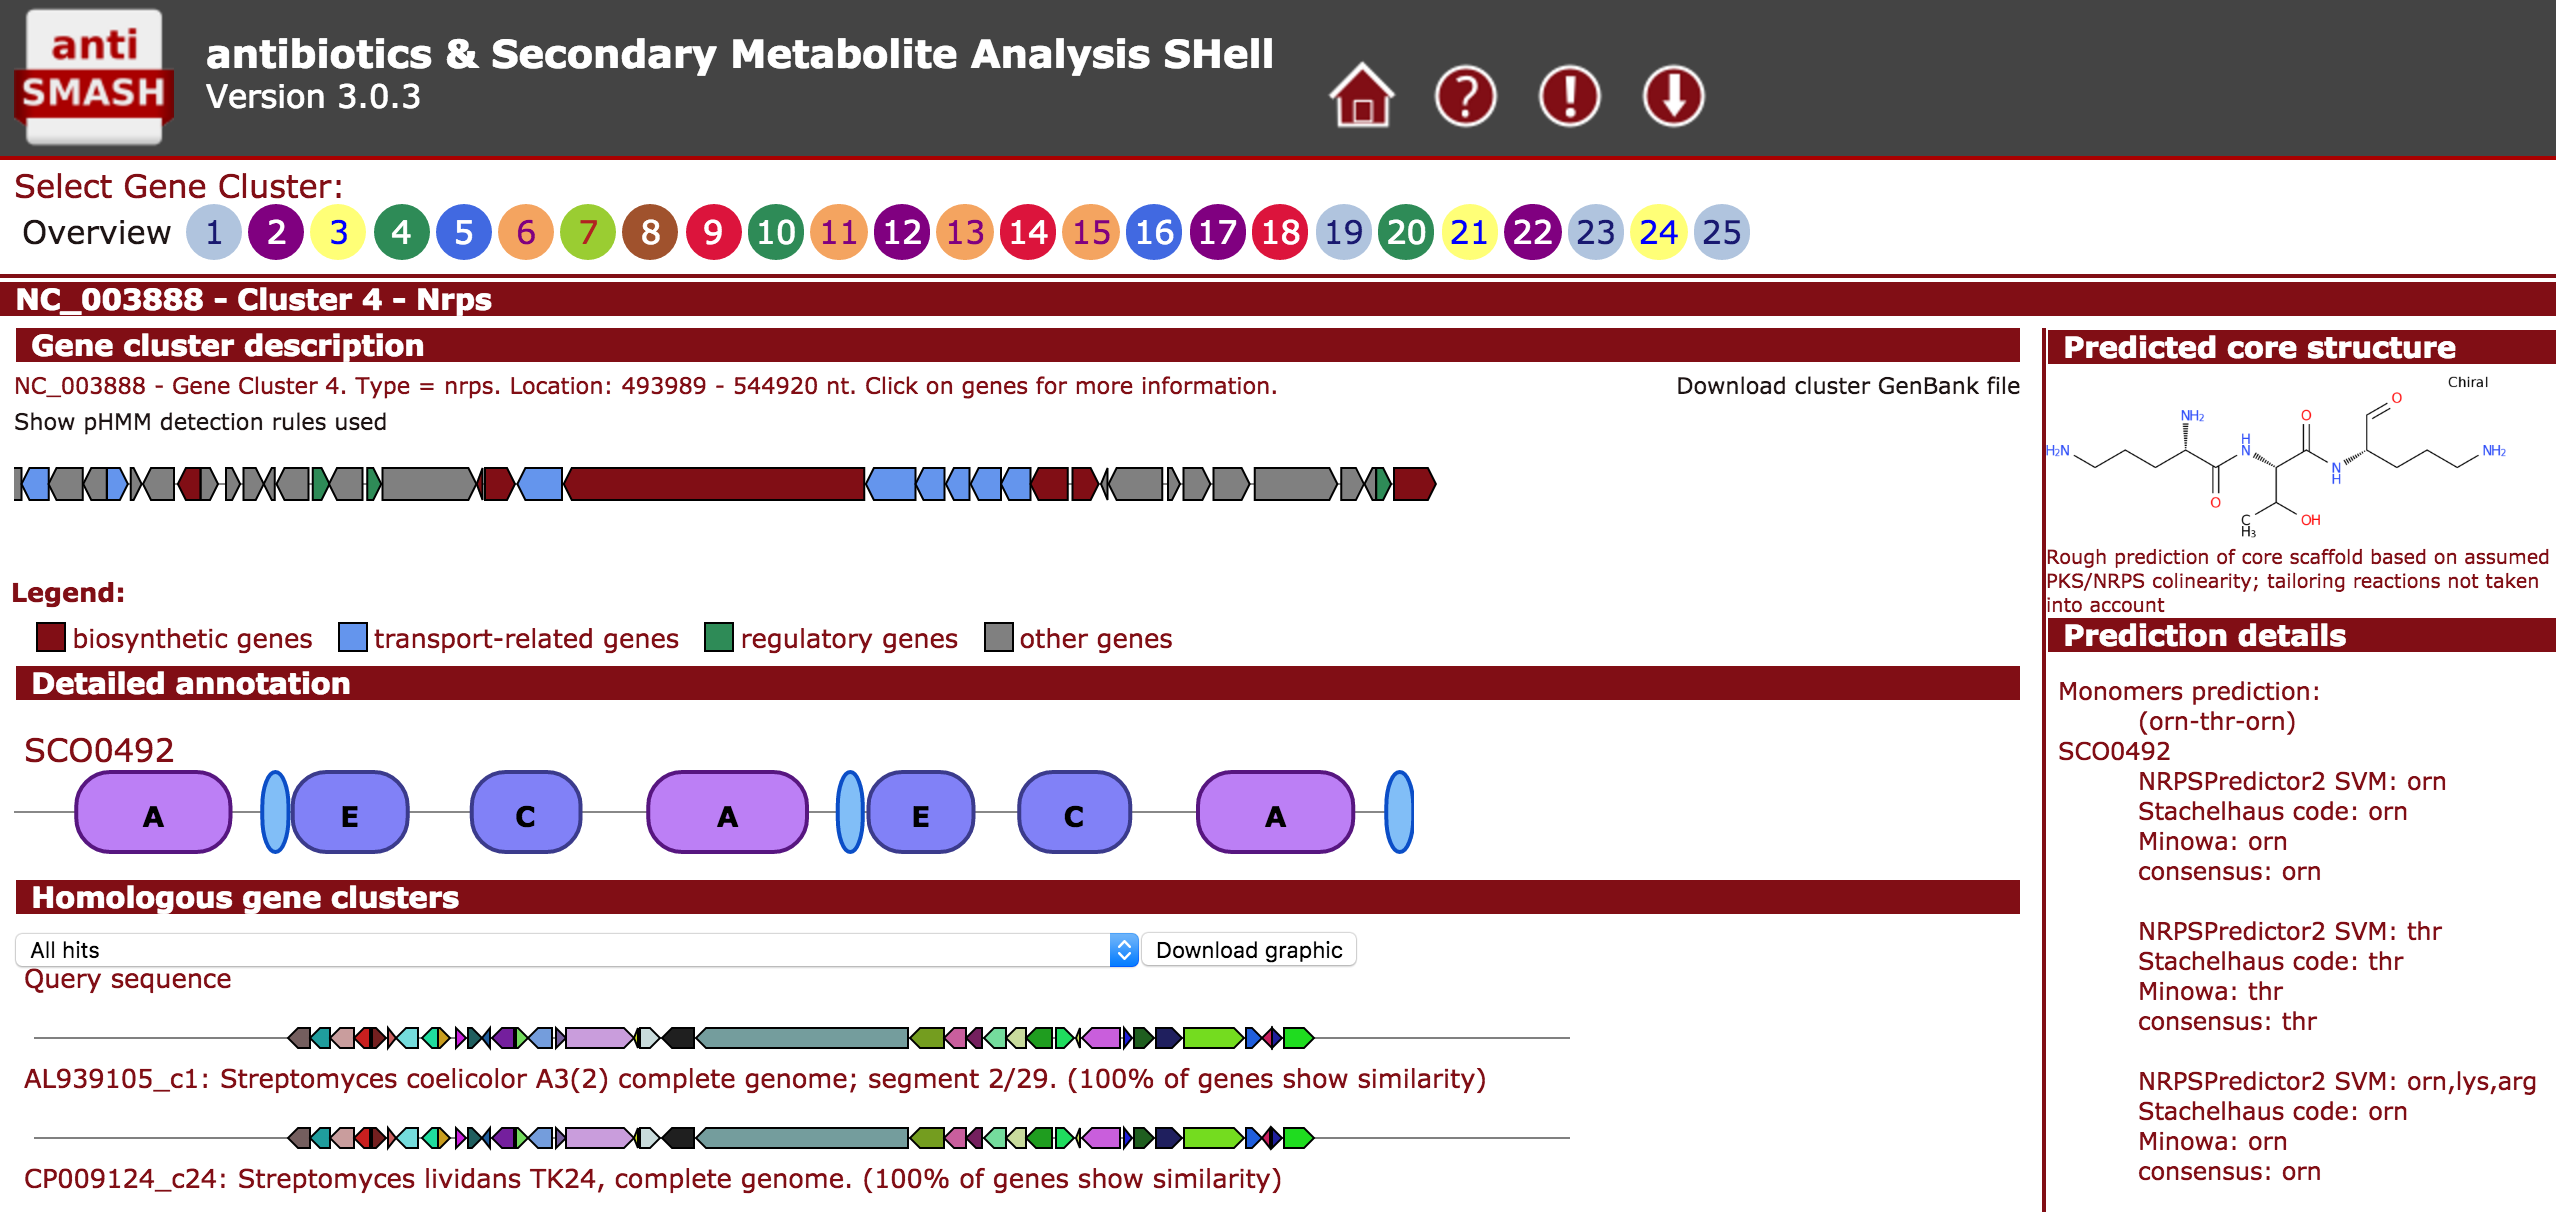
\includegraphics[width=450px]{Figures/bio/Bioinfo/antismash_example.png}
    \caption{\label{antismash_result}Exemple de résultat d'antismash pour un cluster NRPS au sein du génome de Streptomyces coelicolor}
  \end{center}
\end{figure}

\paragraph{}Le gros avantage de Antismash est sa facilité d'utilisation.
Disponible en ligne, il permet l'envoie de génomes ou séquences protéiques pour une analyse sur des serveurs qui lui sont dédiés.
Grâce à ce serveur, l'utilisateur n'a pas de contraintes sur la machine nécessaire au calcul.
Après parfois plusieurs heures de calcul, l'utilisateur reçoit un mail contenant un lien vers ses résultats.
La page de résultats comporte les résultats de tous les clusters qui ont été annotés avec des détails sur chacun des métabolites secondaires attendus.
Cette facilité d'utilisation et la puissance des outils utilisés dans le pipline à permis un grand succès auprès de la communauté.
Le succès à été tel que les auteurs ont du recourir à des listes d'attente avec priorité pour pouvoir obtenir des résultats depuis le serveur dédié.



\subsection{Les bases de connaissances de NRPS}

\paragraph{}Nous allons ici parler de toutes les bases de données qui contiennent des informations à propos des NRPS.
Ces bases servent à préserver les données qui ont été générées par des logiciels de prédiction comme ceux présentés précédemment ou par des analyses biologiques en laboratoire.
Ces données sont en général produites une à une par des chercheurs s'intéressant à un sujet particulier, mais il est très important de les centraliser au sein de grosses bases de connaissance pour pouvoir en tirer des règles générales.

\paragraph{ClusterMine360}
ClusterMine360 est une base de données recensant des clusters de gène NRPS et PKS.
Ce base ne stocke pas vraiment les gènes/protéines mais uniquement les annotations.
Elle pointe vers le NCBI pour toutes les références aux séquences.
Les gènes de la base sont pour la plupart prédits depuis Antismash.
C'est d'ailleurs les résultats de Antismash v1 qui sont affichés pour le détail de chaque cluster.
Malheureusement cette base n'est pas tenue à jour et la dernière news date de 2013.


%· Databases of the thiotemplate modular systems (CSDB) and their in silico recombinants (r-CSDB).
\paragraph{ClustScan Database}
ClustScan Database est une base de données créée à partir des résultats de l'outil de prédiction de NRPS et PKS appelé ClustScan.
Certains clusters ont été vérifiés à la main et sont accompagnés de publications lorsque les utilisateurs de la base les ont ajouté.
Le logiciel permet également la prédiction des structures NRP.
Cependant, la prédiction s'arrête aux structures linéaires et cycliques portées par des domaines de cyclisation.
Ces prédictions de structures NRP sont donc a vérifier avant de les utiliser.


%· Minimum Information about a Biosynthetic Gene cluster
\paragraph{MIBiG, la base de référence des clusters de gènes NRPS/PKS}
MIBiG est une base de données de clusters de gènes de métabolites secondaires, incluant des gènes NRPS accompagnés de leurs annotations.
Les créateurs de la base cherchent la qualité avant la qualité.
En effet, le seul moyen d'entrer des données est de les rentrer à la main en indiquant les sources desquelles proviennent ces données.
Sur le site de MIBiG, les annotations de NRPS sont souvent accompagnées des peptides qui leur correspondent.
Ce lien fort entre clusters de gènes et composé est très intéressant mais n'est entièrement disponible que pour 67 éléments.



\subsection{L'annotation de NRP}

\paragraph{Annotations automatiques depuis l'ADN}
Le séquençage de polymères est une tâche difficile.
C'est pourquoi les protéines ne sont pas directement séquencées mais inférées depuis le séquençage de l'ADN.
Dans le cas des NRP, l'interprétation de l'ADN ne permet que de prédire les séquences protéiques des NRPS.
Il est nécessaire ensuite de comprendre précisément le fonctionnement de ces NRPS pour traduire leur séquence en NRP.
Cependant, comme nous l'avons vu lors des descriptions de logiciels d'analyse de NRPS, cette compréhension ne permet pas encore d'avoir de résultats parfait.
La prédiction ne permet pas de prédire précisément les monomères capturés par les domaines A.
Par exemple il est possible d'obtenir une prédiction un monomère "polaire" sans avoir plus de détails.
Il est également possible d'obtenir des structures monomériques incomplètes, en manquant par exemple les composés capturés par des domaines C starter.

\paragraph{}L'annotation automatique de NRP depuis l'ADN est une méthode très rapide grâce aux technologies récentes de séquençage mais dont les résultats peuvent être incertains voir incomplet.
Lorsque cette technique est utilisée pour connaître la structure d'un NRP, il sera toujours nécessaire de la vérifier d'une autre manière.


\paragraph{Analyse par spectrométrie de masse}
La spectrométrie de masse est une technique physique d'analyse permettant l'identification de structures moléculaires.
Ce procédé est basé sur la mesure de masses moléculaires.
On utilise un échantillon purifié d'une molécule d'intérêt puis on envoie un niveau d'énergie précis afin de casser la molécules en morceaux.
Selon les technologies, une ou plusieurs cassures accompagnées de une ou plusieurs mesures sont effectuées.
L'analyse en résultant permet d'obtenir un spectre contenant différents piques représentant les masses des morceaux obtenus.
Ces masses peuvent ensuite être comparées à des bases de données de masses caractéristiques pour ainsi connaître les composants.
Enfin, à partir des morceaux identifiés, il existe est parfois possible de reconstruire la molécule originelle (tout dépend des technologies qui ont été utilisées).

\paragraph{}Cette méthode permet d'obtenir une reconstruction atomique fiable lorsque toutes les masses sont présentes dans les bases de référence.
Dans ces bases sont par exemple présentes les masses des acides aminés classiques et de leur dérivés proches.
Si la technologie de spectrométrie utilisée casse les molécules au niveau de leurs liaisons peptidiques, la reconstruction permet d'obtenir directement une annotation monomérique de toutes les parties composées d'acides aminés classiques.
Cependant, les NRP étant composés de plus de 500 monomères différents, l'annotation monomérique directement issue des analyses de spectres n'est pas suffisante.
Beaucoup de monomères n'étant pas proche de molécules classiques, ne sont pas répertoriés parmi les masses classiques.
Pour finir l'annotation d'un NRP, il est nécessaire d'avoir recours à un spécialiste du domaine afin qu'il nomme chacun des monomères non annotés.

\paragraph{}Pour résumer, la spectrométrie de masse permet d'avoir accès à des structures atomiques de molécules avec un degré de certitude très élevé.
De plus, contrairement à l'annotation depuis l'ADN, nous sommes certain que la molécule existe puisqu'elle est directement tirée de l'environnement étudié.
Cependant, le besoin d'accès à un expert pour l'annotation et le faible débit de génération de données dû aux purifications nécessaires ne permettent pas une annotation efficace.


\paragraph{Analyse par Résonance Magnétique Nucléaire}
La Résonance Magnétique Nucléaire (RMN) est une technique permettant la détermination de structures moléculaire.
Cette technique exploite la propriété qu'ont certains atomes à émettre un rayonnement lorsqu'ils sont placés dans des champs magnétiques.
Les structures obtenues en sortie sont uniquement atomiques.
Il est donc également nécessaire d'avoir recours à un expert pour effectuer une annotation monomérique.
Cette technique est également très coûteuse de part les équipements nécessaires pour réaliser les analyses ainsi que le temps nécessaire pour créer un cristal capable de convenir à l'analyse.



\subsection{Les bases de connaissance de NRP}

\paragraph{}Les bases de NRP sont très rare en comparaison des bases de NRPS.
Quasiment toutes les bases de NRPS que nous avons précédemment présenté comportent également les structures de NRP prédis.
Cependant, comme nous l'avons déjà dit plusieurs fois ces données ne sont pas toutes fiables.
Beaucoup des structures sont inexactes voir incomplètes dû aux prédictions.

\paragraph{Norine, la base de référence des NRP}
Norine est la base de données de référence pour les peptides non ribosomiques annotés.
Contrairement aux autres bases, c'est une base entièrement dédiée aux NRP.
Tous sont extraits de publications présentant les molécules et déterminant leur caractère NRP.
Chaque molécule entrée dans la base est accompagné de sa structure monomérique (et parfois de se structure atomique).
Depuis 2015, la base de donnée est entièrement ouverte aux contributions exterieurs.
En quelques clics et en appuyant sa soumission par des articles de preuve de la voie de synthèse, toute personne peut soumettre de nouvelles entrées.
Les structures présentes dans cette base sont sures, ce qui est un gros avantage comparé aux prédictions présentées jusqu'à présent.
Cependant, le processus d'ajout de nouvelles entrées, strict pour préserver la qualité, ne permet d'ajouter de nouvelles entrées par centaines.
Soulignons tout de même le travail effectué par les auteurs initiaux qui ont entré plus de 1200 annotations à la main.


\paragraph{MIBiG}
Retour sur MIBiG car c'est la seule base hors Norine encore active et contenant des annotations vérifiées de NRP.
Comme nous l'avons déjà dit lors de la présentation de cette base, MIBiG est une base surtout dédiée à l'annotation de NRPS.
Les annotations de NRPS sont accompagnées d'informations sur les peptides produits.
Ces informations peuvent être de deux types.
Soit l'organisme est connu comme producteur d'un NRP dont on connait la structure et l'annotation de NRPS peut être vérifiée.
Dans ce cas, la structure présente dans MIBiG est exacte même si on ne sait parfois pas quels gènes sont venu ajouter/modifier des morceaux du NRP.
Soit le NRP est une prédiction depuis le cluster de gènes.
Dans ce cas, il se peut qu'il ne soit que partiel et potentiellement incorrect.















\chapter{Smiles2Monomers : Des atomes vers les monomères}

\section{Introduction des principes}

\subsection{Pourquoi chercher les structures monomériques des NRP ?}

\paragraph{}L'un des principes fondamentaux lorsque l'on cherche à comprendre quelle est l'activité d'une molécule,
est de dire que cette activité a une relation forte avec la structure de cette molécule. Ce principe est appelé la
``Relation Quantitative Structure à Activité'' (en anglais : Quantitative Structure-Activity Relationship (QSAR))
\cite{patani_bioisosterism:_1996,leach_molecular_2001,helma_predictive_2005}.
Par structure, il ne faut pas uniquement entendre conformation 2D ou 3D de la molécule mais également toutes les
propriétés physico-chimiques qui résultent des atomes et liaisons présents.
Lorsque l'on cherche à décrire l'activité d'une molécule on étudie donc sa structure et l'on part du postulat que
deux structures semblables ont une activité semblable. Pour prédire l'activité d'une molécule il est donc nécessaire
de comparer sa structure avec des structures dont on connaît déjà l'activité. Il existe beaucoup de techniques\{TODO Refs nécessaires\} de
comparaison mais elles ont toutes un point commun : Plus la comparaison de structure inclut de propriétés et plus
elle est précise mais difficile a effectuer. Le but est donc d'essayer d'étudier des propriétés pertinentes et
faciles à comparer.

\paragraph{}Dans le cas des NRP, l'analyse des activités revient donc à chercher les ressemblances et les différences
entre la molécule étudiée et celles dont on connaît déjà la ou les activités. Beaucoup d'approches QSAR classiques
sont applicables à partir du moment où elles ne nécessitent que l'étude de la structure atomique mais nous pouvons
également nous appuyer sur l'information apportée par la structure monomérique de ces NRP. En 2012\cite{abdo_new_2012}
puis 2014\cite{abdo_prediction_2014}, Abdo et al. publiaient la pertinence de l'analyse d'activités de NRP à partir
de cette structure en utilisant respectivement des fingerprints et des réseaux bayesiens. L'avantage d'utiliser la
structure monomérique au lieu de la structure atomique est la rapidité d'analyse. Là où une comparaison chimique
dépend du nombre d'atomes présent dans les molécules (plusieurs centaines), la comparaison monomérique de NRP est
dépendante du nombre de monomères (une vingtaine au maximum).

\paragraph{}TODO : Conclusion des deux paragraphes du dessus.




\subsection{Formalisation du problème}

\subsubsection{Formalisation générale}

\paragraph{}Résumons la situation. Les NRP sont des molécules polymères assemblées à partir d'un nombre de briques
de bases monomériques finies. Lors d'un séquençage de ces molécules, nous avons accès à la structure chimique de
ces composés mais pas toujours à leur structure monomérique. Cette structure nous intéressant particuliérement,
nous aimerions pouvoir remonter automatiquement depuis la structure chimique vers la structure monomérique.

\paragraph{}En formalisant cette demande d'un point de vue informatique, nous pouvons dire que nous aimerions avoir
un programme qui prend en entrées une structure chimique que l'on sait être un NRP ainsi qu'une liste de monomères
finie que l'on sait composer les NRP, pour produire une sortie qui nous permet de dire quels monomères sont présents
dans le polymère en sachant à quels atomes ils sont rattachés.

\paragraph{Figure s2m}





\subsubsection{Les problématiques existantes}

\paragraph{}TODO : Réécrire sous la forme 2 techniques monos->poly ou polys->monos + figure

\paragraph{}Une technique appelée CHUCKLES\cite{siani_chuckles:_1994} et décrite en 1994 correspond parfaitement à
ce que nous recherchons. Dans des buts de requêtage et de compression, les auteurs avaient besoin d'un moyen de
passer rapidement de la représentation monomérique à la représentation atomique et inversement. La partie ``inverse''
(Back-Translation dans l'article) part de la liste des 20 acides aminés standards (sans leurs atomes d'hydrogène)
et les recherche un à un de manière exacte en commençant par les plus gros. La recherche des monomères se fait
de manière indépendante en utilisant un format appelé SMARTS\{TODO Ref\} qui permet de faire des recherches par des
algorithmes d'isomorphisme de sous graphe (voir sous partie suivante pour plus de détails). Cette technique fonctionne
parfaitement avec les 20 acides aminés standards tant qu'ils ne sont pas transformés au sein de la molécule d'arrivée.
Cependant, dans le cas des peptides non-ribosomiques, le nombre de monomères s'élève à plus de 500 dont certains
étant très ressemblants. Dès que ces monomères très ressemblants sont intégrés au NRP (et donc qu'ils ont été
modifiés par les liaisons) il devient alors impossible à partir d'un algorithme simple d'être certain de trouver
la bonne transformation (Et ce même si elle est possible). Cette méthode est donc une bonne base de travail pour
créer notre outil mais n'est pas suffisant pour outrepasser la complexité des molécules que nous souhaitons traiter.

\paragraph{}Une seconde possibilité pour séparer une molécule en sous-composants est de choisir des règles de
découpe de liens en ciblant certaines zones d'intérêt. Le logiciel molBLOCKS\cite{ghersi_molblocks:_2014} utilise
cette stratégie. Le logiciel découpe non pas une mais un ensemble de molécules d'intérêt selon les règles définies
jusqu'à ne plus pouvoir ou jusqu'à atteindre une limite minimale de taille de fragments (fixée par l'utilisateur).
Le logiciel analyse ensuite la fréquence des fragments sur l'ensemble des molécules pour déterminer les fragments
qui ont le moins de chance d'être artificiellement créés et ainsi les considérer comme les monomères réels. Cette
méthode à pour gros avantage de ne pas prendre de base de donnée de monomères comme prérequis et propose une
manière élégante de les retrouver. Cependant rien ne garantit que les monomères créés ne sont pas artificiels.
De plus, les monomères rares dans la base de données ne généreront pas de fragments avec une suffisamment grande
redondance pour être considérés comme réels. Enfin, si les règles de découpe sont mal choisies, les fragment générés
n'auront aucune signification biologique.

\paragraph{}Sous techniques
\paragraph{}SMARTS+variants (ambit-smarts)
\paragraph{}Recherche de 1 molécule dans une autre (SMSD (MCS), .


\paragraph{Conclusion}Séparation en deux sous problèmes







\subsubsection{Des molécules aux graphes}

\newtheorem{definition}{Definition}
\begin{definition}\textbf{Graphe :}
 Un graphe est une représentation mathématique d'un ensemble d'objets où chacun des objets est appelé un sommet et
 chaque relation entre deux objets est représentée par un lien entre les deux sommets représentant ces objets.
\end{definition}

\paragraph{}En suivant cette définition, nous allons pouvoir représenter nos deux type de structure sous la forme de
graphe.

\paragraph{Structure chimique :}La structure chimique d'une molécule, c'est à dire ses atomes reliés par ses liaisons
chimiques se représente immédiatement. Les atomes seront nos sommets de graphes et les liaisons les arêtes. Je rajouterai
comme petite subtilité que les hydrogènes ne seront pas représentés comme sommets mais inclus directement dans le sommet
de l'atome plus lourd sur lequel il est lié. Par exemple pour représenter CH3NH2, seuls deux sommets seront définis :
(CH3) et (NH2). Ces deux sommets seront reliés par une arête représentant la liaison entre le C et le N. Remarque :
cette représentation exclue la possibilité d'avoir un graphe pour le dihydrogène.

\paragraph{Structure monomérique :}La structure monomérique, c'est à dire les monomères et leur liaisons chimiques se
représentent tout aussi immédiatement. Les monomères seront les sommets et les liaisons les arêtes des graphes
monomériques.

\paragraph{}Dès à présent dès que je parlerai de molécules quelles qu'elles soient, je parlerai par abus de langage
du graphe représentant la structure atomique de cette molécule. Il en sera de même pour la structure monomérique.



\subsubsection{Formalisation en problèmes de graphes}

\paragraph{}Comme expliqué plus haut le problème de recherche de sous composants d'un polymère peut être divisé en deux
plus petit problèmes : un problème de recherche de monomères et un problème de placement des monomères trouvés. Traitons
donc séparément ces deux problèmes.

\paragraph{Recherche de monomères}Rechercher un monomère dans un polymère revient à rechercher un petit graphe atomique
$S$ dans un plus gros graphe $G$. Deux cas sont alors possibles, soit nous recherchons à trouver exactement $S$ dans
$G$, soit nous cherchons une approximation de $S$ dans $G$. Dans le premier cas, nous allons nous intéresser à l'
``Isomorphisme de Sous-graphe'' (en anglais Subgraph Isomorphism (SI)). Dans le second cas, nous nous intéresserons au
``Sous-graphe Maximum Commun'' (en anglais Maximum Common Subgraph (MCS)). Les recherches de SI ou de MCS ont toutes
deux été prouvées NP-Complet mais pour chacun des problème il existe des algorithmes rapides en pratique pour des graphes
aux propriétés particulières dont nous parlerons dans la sous partie suivante.

\paragraph{Placements des monomères}Une fois les monomères détectés, il est nécessaire de prendre une décision pour les
parties du polymère où plusieurs d'entre eux ont été détectés au même endroit. L'objectif est donc de faire un choix entre
les différents morceaux possibles afin de chercher à ne garder que les pièces non chevauchantes qui permettent de couvrir
au mieux le polymère (Si possible totalement). Ce genre de méthode est appelée pavage sans recouvrement. Cette étape
donnant accès à un lien direct entre atomes et monomères, une étape de contraction de graphe permettra d'obtenir le graphe
monomérique.




\subsection{Isomorphisme de Sous-graphe et Sous-graphe Maximum Commun}

\paragraph{}Nous avons vu que nous pouvions faire correspondre deux problèmes de graphes différents avec notre problème
de recherche de monomère. Le but de cette partie est d'étudier les différents algorithmes existant pour chacun de ces
problèmes

\subsubsection{Sous-graphe Maximum Commun : définition}

\paragraph{}Commençons par définir clairement le sous graphe maximum commun.

\begin{definition}\textbf{Sous-graphe Maximum Commun :}
  Soient deux graphes $G(V, E)$ et $G'(V', E')$, composés respectivement de $V$, $V'$ leur ensembles de noeuds et de $E$, $E'$
  leur ensembles d'arêtes. Soit $f(V, V')$ une fonction de comparaison qui retourne vrai si le sommet de $V$ passé en paramètre
  est identiques au sommet
  de $V'$. Le Sous-graphe Maximum Commun est défini comme un graphe $H(M, N)$ avec $M$ et $N$ construits comme suit. $\forall
  s(u,v)\in~M, f(u, v)$ et $|M|$ est  maximal. $a(s, t) \in N$ ($s \in M$ et $t \in M$) avec $s_1$, $s_2$ les sommets de
  $G$ et $G'$ composants $s$ et $t_1$, $t_2$ les ceux composants $t$, ssi $\exists v \in V$ entre $s_1$ et $t_1$ et $v' \in
  V'$ entre $s_2$ et $t_2$.
\end{definition}

\paragraph{}TODO : Image de MCS



\subsubsection{Isomorphisme de Sous-graphe : définition}

\paragraph{}De la même manière que pour le MCS, définissons précisément ce qu'est l'Isomorphisme de Sous-graphe

\begin{definition}\textbf{Isomorphisme de Sous-graphe :}
 Soient un graphe $G(V, E)$ et un graphe requête $R(M, N)$ plus petit que $G$. Un Isomorphisme de Sous-graphe de $R$ sur $G$ est
 une association isomorphe d'une sous partie de $G$ avec $R$. Définissons une fonction booléenne $f(a, b)$ d'association
 de noeuds qui est vraie lorsque les noeuds $a$ de $R$ et $b$ de $G$ sont isomorphes. Un SI peut alors être défini par :
 \begin{itemize}
  \item $\forall m \in M, \exists v \in V$ tel que $f(m, v)$ est vrai. On appel alors $A(m, v)$ l'association de m et v.
  \item $\forall \{A(a, b) , A(c, d)\}$ si $\exists n \in N$ reliant $a$ et $c$ alors $\exists e \in E$ reliant $b$ et $d$.
 \end{itemize}
\end{definition}


\paragraph{}TODO : Image de SI


\paragraph{TODO}Conclure la section par la décision de isomorphisme + tiling

\section{Algorithmes}

\subsection{Isomorphisme de sous graphe}

\paragraph{}La première partie Smiles2Monomers doit rechercher l'ensemble des monomères au sein d'un polymère cible.
Comme nous l'avons vu dans l'état de l'art, ce problème transformé en problème de graphe est un problème d'isomorphisme de sous
graphe.
Dans cette partie nous allons présenter en détail l'algorithme classique de recherche de SI nommé VF2 en l'étendant à des graphes
labellés.
Puis nous montrerons en quoi les labels des noeuds du graphes influencent le temps de calcul afin en déduire une méthode de
recherche efficace.

\subsubsection{L'algorithme originel VF2}

\paragraph{}Comme nous l'avons déjà évoqué dans l'état de l'art de cette partie, l'algorithme VF2 permet d'effectuer des
isomorphisme de graphe ou de sous-graphe non labellés d'un graphe $G$ sur un graphe $H$.
Écrivons l'algorithme tel qu'il est décrit dans l'article d'origine :

\paragraph{}
  \begin{algorithm}[H]
    \caption{Algorithme VF2 pour graphes non labellés}
    \KwData{Un graphe $G(V,E)$ et un graphe $H(V',E')$ avec $|V| \leq |V'|$ et $s$ un état contenant les mappings déjà effectués
    entre les deux graphes}
    \KwResult{Un mapping entre les éléments de $V$ et une sous partie des éléments de $V'$ telle que $H$ soit un isomorphisme de
    sous graphe de $H$}
    
    \uIf {$s$ contient un mapping de tous les éléments de $V$} {
      \KwRet $Mapping(s)$\;
    } \uElse {
      \uIf {$Mapping(s)$ est vide} {
	$P \gets$ ensemble des $p(x,y)$ tq $x \in V$ et $y \in V'$ \;
      } \uElse {
	$P \gets$ ensemble des $p(x,y)$ tq $x \in V$, $y \in V'$ et $\exists p(a,b) \in Mapping(s)$ tq $a$ et $x$ soient voisins dans
	$G$ et $b$, $y$ voisins dans $H$ \;
      }
      
      \For {$p \in P$} {
	$s' \gets p \cup s$\;
	\If {$VF2(G, H, s') != \emptyset$} {\KwRet $Mapping(s')$\;}
      }
      
      \KwRet $\emptyset$ \;
    }
  \end{algorithm}

\begin{figure}
  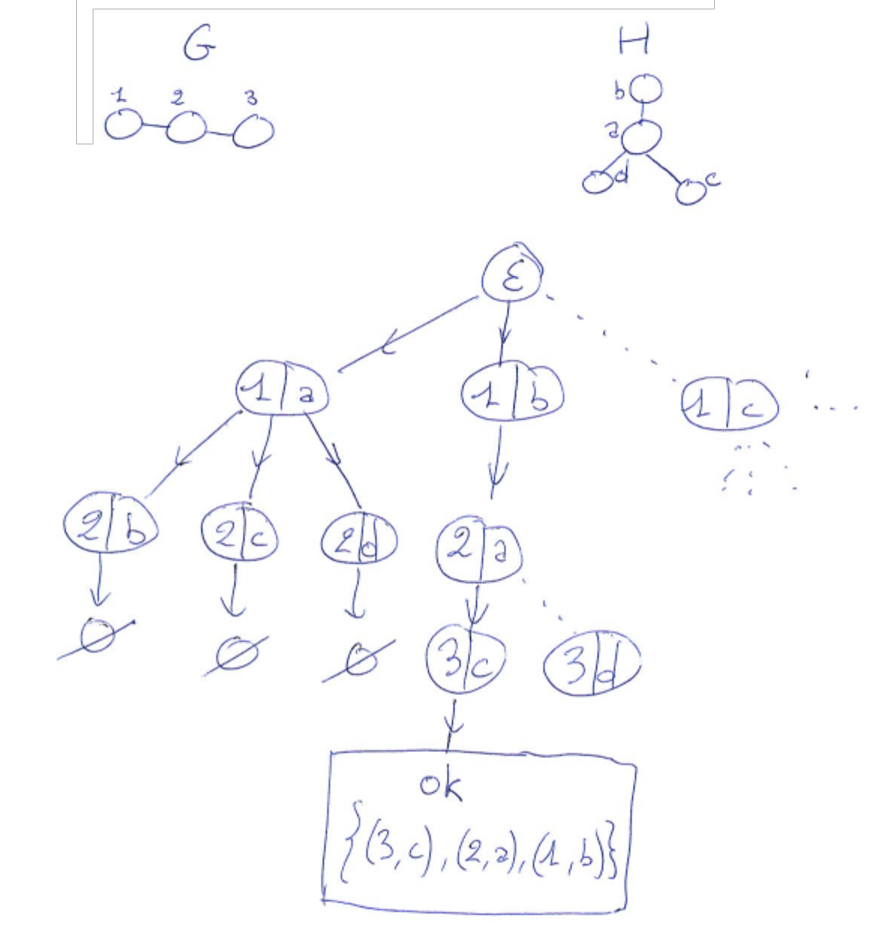
\includegraphics[width=200px]{Figures/s2m/recherche/VF2.pdf}
  \caption{\label{vf2}Représentation sous forme d'arbre d'une recherche de d'isomorphisme de sous graphe par l'algorithme VF2}
\end{figure}

\paragraph{}Expliquons cet algorithme en utilisant le schéma \ref{vf2}.
A la première étape nous nous trouvons avec un ensemble vide de noeuds pairés de $G$ et $H$.
Nous générons donc toutes les possibilités d'assemblage entre tous les noeuds des deux graphes (Il est à noter que l'algorithme
est décrit de cette façon dans l'article mais qu'il n'est nécessaire de générer que les couples à partir d'un seul noeud de $G$
et de l'ensemble des noeuds de $H$.
Une fois ces assemblages créés, nous les parcourons tous en appelant récursivement la fonction.
Dans l'exemple le premier appel récursif est effectué après avoir assemblé '1' à 'a'.
Cette voie est sans issue car quel que soit l'assemblage entre '2' et un noeud de $H$, plus aucun couple de voisins ne pourra être
généré.
En effet pour générer l'ensemble $P$ il est nécessaire de regarder tous les voisins de 'b' alors que le noeud ne possède plus
de voisins hors de $s$.
Une fois toutes les tentatives échouées, l'algorithme remonte dans l'arbre et change l'association '1'-'a' pour l'association
'1'-'b'.
Récursivement l'algorithme conclut à un isomorphisme {(1,b);(2,a);(3,c)}.

\paragraph{}En l'état l'algorithme VF2 ne permet de reconnaître qu'un seul et unique isomorphisme.
On peut modifier simplement l'algorithme afin de récupérer tous les isomorphismes en ne retournant pas une fois que l'un d'eux est
trouvé mais en l'enregistrant dans un ensemble puis en continuant l'exploration de l'arbre jusqu'au bout.
Vu que tout l'arbre est exploré à chaque recherche, l'algorithme est exponentiel.
Pour être plus précis il est en $O(n^m)$, donc pas calculable dans les pires des cas.

\begin{figure}
  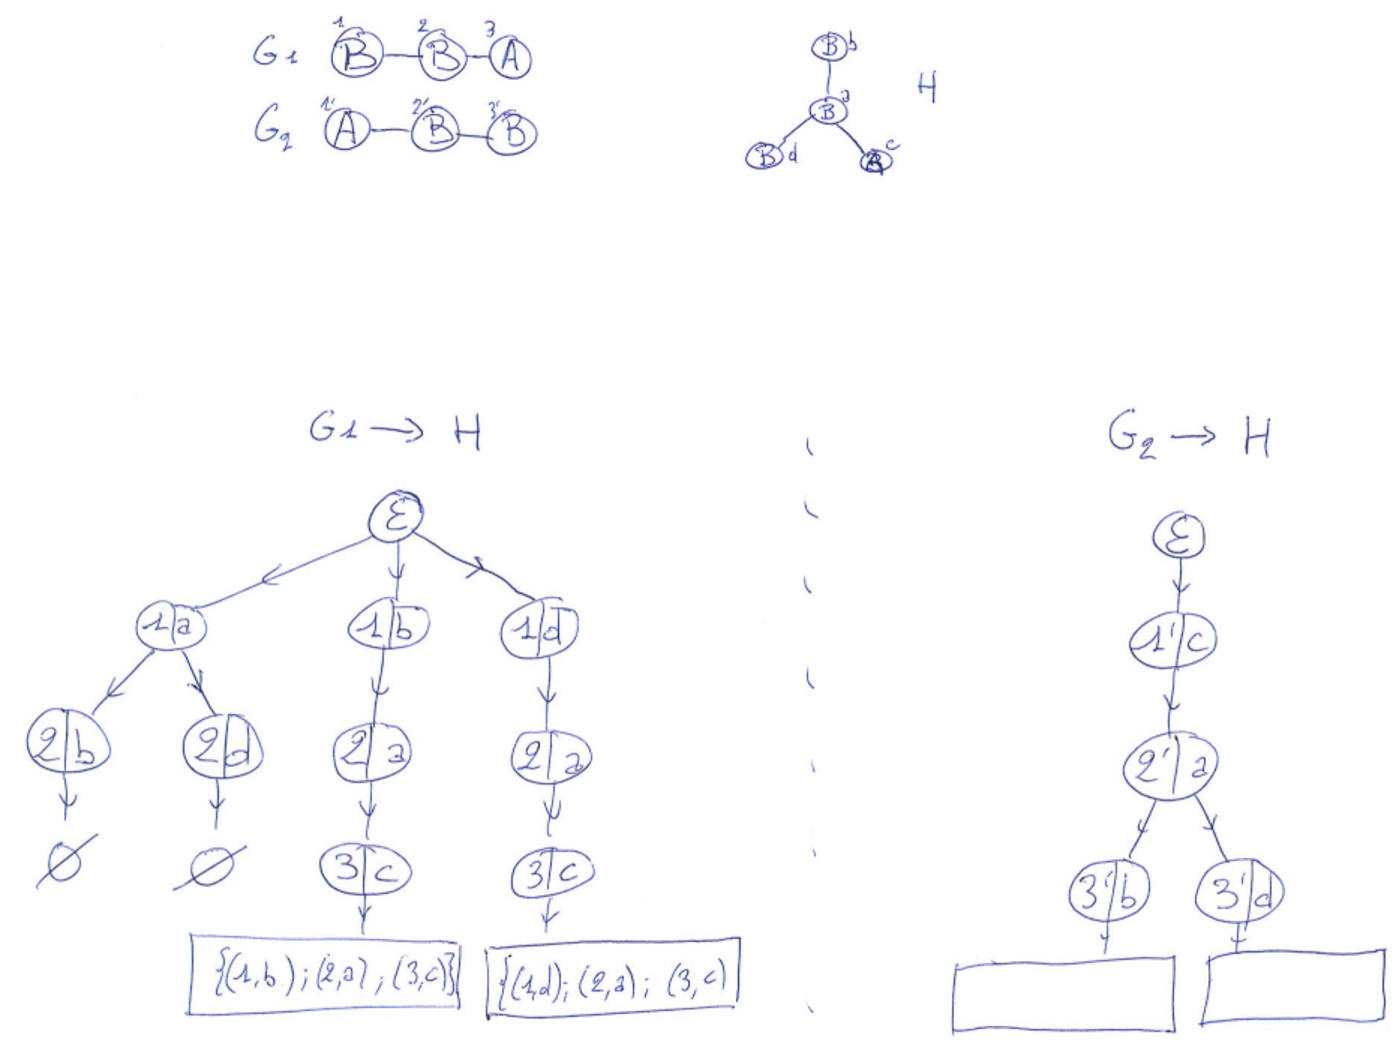
\includegraphics[width=200px]{Figures/s2m/recherche/VF2_labels.pdf}
  \caption{\label{vf2_labels}Représentation sous forme d'arbre de recherches pour l'algorithme VF2 appliqué aux graphes labellés}
\end{figure}

\paragraph{}Intéressons nous maintenant aux graphes labellés.
On peut modifier l'algorithme VF2 pour qu'il ne prenne en compte que les paires de noeuds possédant le même label.
Prenons à nouveau notre exemple précédent en labellant avec A et B les noeuds.
Sur la figure \ref{vf2_labels}, on peut voir la recherche d'un graphe $G$ composé de 2 noeuds A et un noeud B au sein d'un graphe $H$
composé d'un branchement supplémentaire contenant un noeud B.
Sur ce graphique nous avons représenté deux cas de recherche selon l'ordre dans lequel nous prenons $G$.
Nous pouvons remarquer que dans les deux cas, la taille de l'arbre est bien plus faible que pour un graphe non labellé.
Les labels des noeuds font office de filtres de recherche et permettent d'accélérer fortement la recherche.
On voit également que la recherche est d'autant plus rapide que l'on choisi prioritairement les noeuds avec des labels de faible
fréquence.

Là où l'algorithme général VF2 était en $O(n^m)$, la complexité est ici réduite dans le pire des cas à $O(k^n)$ où $k$ est le
comptage du nombre de noeud du label le moins filtrant.
La taille de l'arbre de recherche est diminué par la sélectivité des labels de noeuds.
Pour optimiser la recherche, nous devons donc étudier la façon dont nous représentons les molécules afin d'avoir une sélectivité
la plus grande possible.

\subsubsection{Sélectivité d'un noeud}

\paragraph{}Premièrement, attachons nous à la représentation la plus basique possible d'un graphe chimique (atome=noeud,
liaison=arête). Dans cette représentation, nous pouvons considérer chaque label comme étant le nom de l'atome du noeud (Voir
figure \ref{representations}, première partie). Évidemment, les hydrogènes sont les atomes les plus représentés et ne filtrent
pas les recherches par eux-mêmes. Cependant, ils sont un bon moyen de donner des précisions sur l'atome auquel ils sont liés.
Ainsi, trouver un $CH_{3}$ ou un $CH$ donne une information différente sur la topologie.
En prenant en compte la remarque précédente nous avons créé une seconde représentation qui compresse les hydrogènes à l'intérieur
des noeuds représentant les atomes plus lourds.
Ainsi, plusieurs labels différents peuvent
désormais être créés pour un même atome et ce, en fonction de ses compagnons hydrogènes (Voir figure \ref{representations},
seconde partie). Par exemple $NH_2$, $NH$, $N$ sont les
trois labels variant depuis l'ancien label unique $N$ qui était accompagné de voisins hydrogènes. Les labels sont plus nombreux et
leur fréquences à la fois moins élevée et plus homogène, ce qui permet de les rendre plus sélectifs.

\begin{figure}
  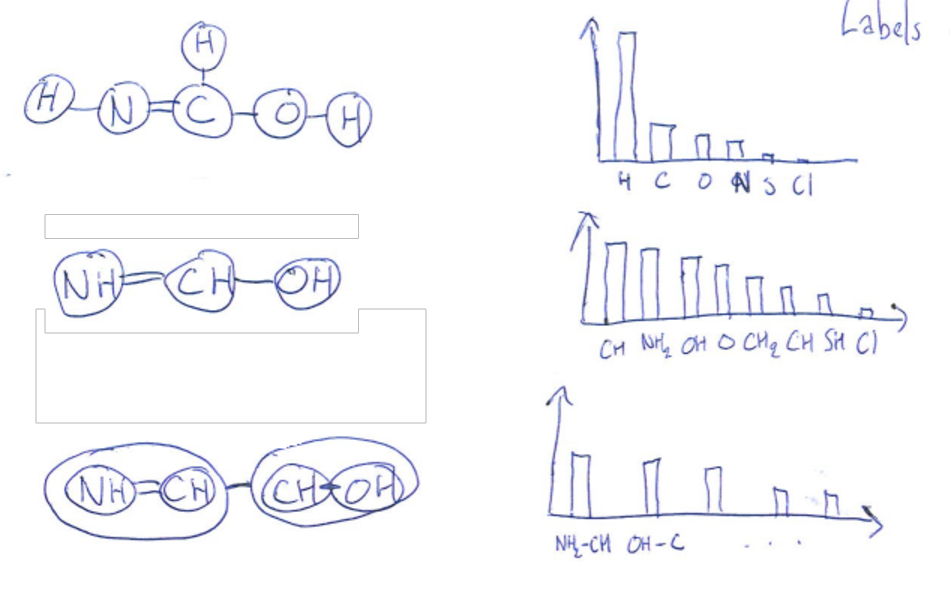
\includegraphics[width=300px]{Figures/s2m/representations/all_tmp.pdf}
  \caption{\label{representations}Manque fréquences et titres dans l'image}
\end{figure}

\paragraph{}Globalement, plus le nombre de labels est élevé et leur fréquences homogènes et moins l'algorithme VF2 aura de
difficultés à effectuer un isomorphisme. En effet la lenteur qui peut venir de cet algorithme est dû au nombreux chemins qu'il
peut prendre lors de l'exploration.

\paragraph{}Cherchons encore à augmenter la sélectivité des labels en augmentant leur nombre. A partir d'un graphe $G$ il est
possible de représenter ses relations d'adjacence au sein d'un second graphe $L$. Pour cela, deux noeuds voisins de $G$ sont
représentés dans $L$ comme un seul noeud. Chaque ancienne arrête devient un noeud et chaque ancien noeud devient une multitude
d'arête (une clique entre tous les nouveaux noeuds représentant les anciennes arête de cet ancien noeud). Nous étendons le 
raisonnement pour les labels en disant que le label d'un noeud du nouveau graphe est la composition des labels des anciens
noeuds ainsi que de l'arité entre ces deux noeuds (Dans notre cas, les labels sont mis dans l'ordre lexicographique pour ne pas
avoir deux labels possibles à partir des labels d'origine)(Voir figure \ref{representations},
troisième partie). Un tel type de graphe est appelé line graph\cite{orlin_line-digraphs_1978}. L'un des
gros avantage de cette représentation est d'inclure directement dans les labels des noeuds ce qui touche à l'arité entre noeuds.
La fonction
de recherche n'aura donc plus du tout à s'attarder sur les liens mais uniquement sur les noeuds. De plus, transformer les graphes
de cette manière nous permet de répondre à la volonté d'augmentation du nombre de labels. Là où la représentation précédente
pouvait avoir $n$ labels différents, celle-ci pourra générer plus de $n^2$ ($3n^2$ si on compte tous les type de liaison entre
noeuds).

\paragraph{}Le raisonnement des line graphe peut être étendu récursivement. On peut ainsi créer des line-graph de line-graph.
Cependant cela pose plusieurs problèmes de répéter cette opération dans notre cas. Certains graphes vont diminuer de taille
jusqu'à disparaître complètement (ce qui est peu pratique pour la comparaison) alors que d'autres vont grossir de plus en plus
et ajouter de plus en plus de phases de comparaison de labels et d'étapes dans l'algorithme VF2. Pour ces raisons nous avons
choisi de n'effectuer qu'une seule étape de line-graph.

\begin{figure}
  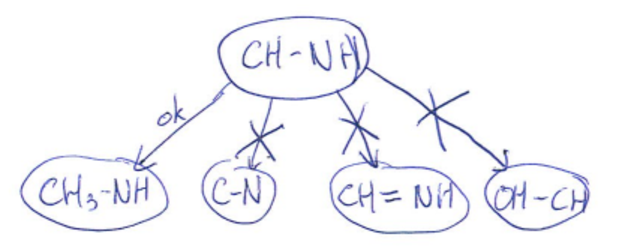
\includegraphics[width=200px]{Figures/s2m/recherche/matching.pdf}
  \caption{\label{label_matching}Exemple de fonctionnement de la fonction de matching de labels}
\end{figure}

\subsubsection{Indexation des monomères}

\paragraph{}Connaissant la sélectivité pour un label, nous cherchons désormais à savoir l'ordre dans lequel il faut rechercher
un motif afin de minimiser le temps de recherche.
Nous appellerons \textbf{motif} le graphe compressé que nous allons vouloir retrouver dans un plus
grand graphe. Définissons également une \textbf{chaine} comme étant un motif plus un ordre dans lequel parcourir ce motif. Ainsi,
on peut avoir plusieurs chaînes représentant le même motif mais avec des ordres de parcours différents. Ce que nous appellerons
indexation sera donc la phase de recherche d'une chaîne pour représenter chaque motif d'intérêt en essayant de minimiser le temps
que prendra la recherche de cette chaîne. Pour la recherche de monomères dans
des peptides non ribosomiques, la phase d'indexation revient donc à choisir, pour chaque monomère, l'ordre dans lequel nous allons
rechercher les noeuds du graphe le représentant. Ainsi on peut voir que quelque soit la chaîne représentant le graphe, le même
motif sera toujours recherché. La seule différence sera la rapidité d'exécution de la recherche. Les deux sections suivantes
s'attarderont à la recherche de chaînes performantes (ie les plus rapide) lors la recherche d'un motif.


\subsubsection{Indexation gloutonne}

\begin{figure}
  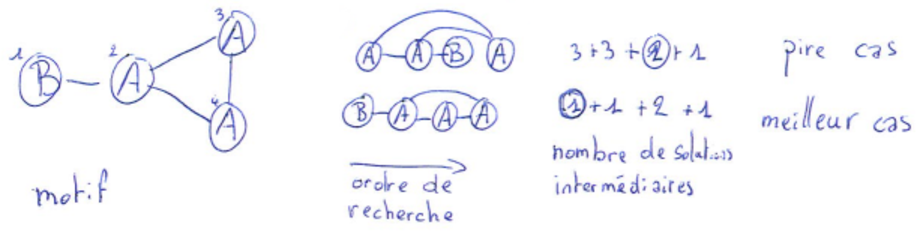
\includegraphics[width=300px]{Figures/s2m/indexation/chaine_fail.pdf}
  \caption{\label{chaine_fail}Deux exemple de chaîne pour un motif simple}
\end{figure}

\paragraph{}Une bonne chaîne est donc une chaîne rapide mais a quoi ressemble une telle chaîne ? Déterminons quel(s) critère(s)
simple(s) nous permettent de supposer qu'une chaîne est bonne. Avec ce ou ces critères nous pourrons ensuite déterminer un
moyen d'ordonner les noeuds de manière gloutonne. Partons de l'exemple présenté sur la figure \ref{chaine_fail}. A gauche est
dessiné un motif simple suivi de deux chaînes pouvant le représenter (lecture de l'ordre des chaînes de gauche à droite). Pour
la première chaîne, en partant du motif ne contenant qu'un A, on obtiendra 3 isomorphismes. En étendant ces chaînes à deux A
voisins, on conserve toujours trois isomorphismes puis deux en ajoutant B et enfin un seul avec le dernier A. Au total on aura
étendu 9 isomorphismes durant la recherche. En regardant maintenant la seconde chaîne, on se rend compte que le nombre de ces
isomorphismes intermédiaires est bien plus faible grâce à la sélectivité du B recherché en tout premier (5 isomorphismes
intermédiaires sont étendus). La différence décisive entre les deux chaînes est donc le moment où le noeud avec un label sélectif
est recherché. Si le noeud B est recherché dès le début, la solution est ``ancrée'' sur une base solide et ne risque pas de 
créer trop de solutions intermédiaires qui devront toutes être analysées pour passer à l'étape suivante. On peut dire qu'un noeud
est plus sélectif qu'un autre à partir du moment où sa fréquence d'apparition dans les molécules étudiées est moins élevée.

\paragraph{Labels fréquents}

\begin{figure}
  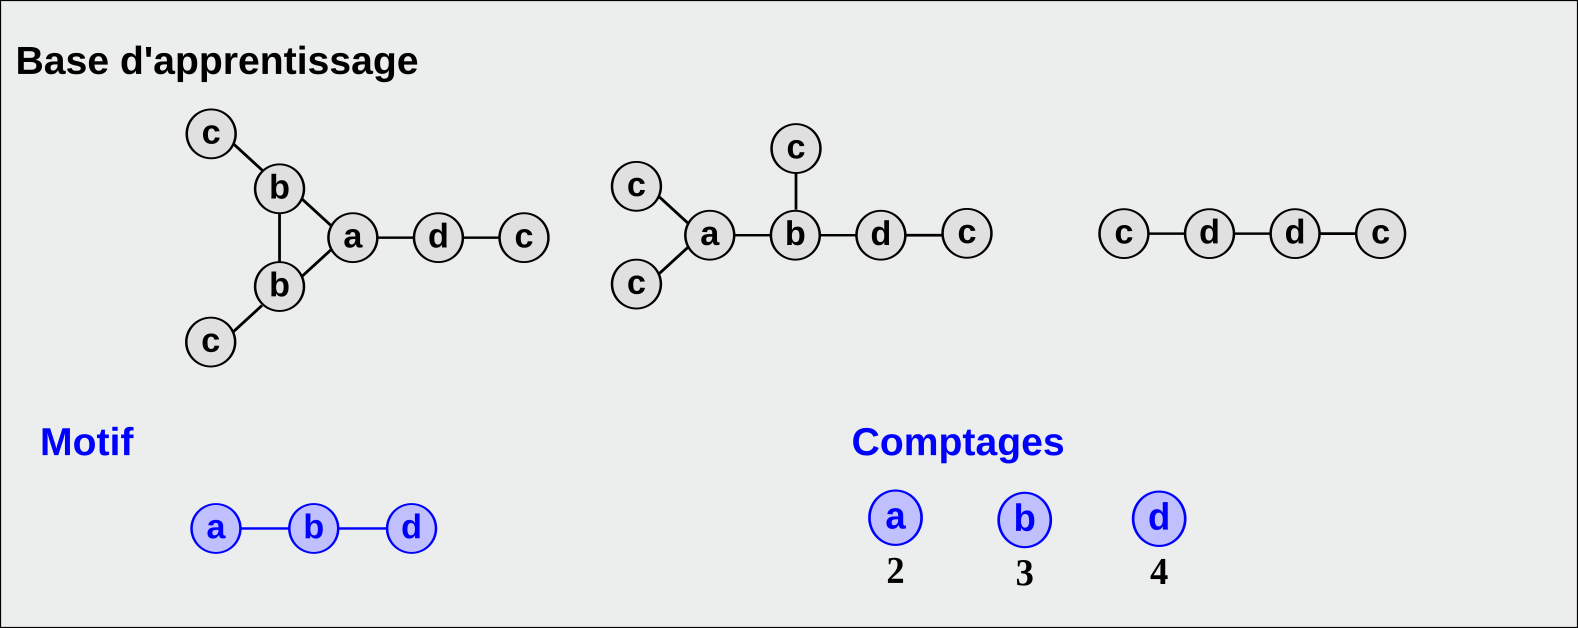
\includegraphics[width=300px]{Figures/s2m/indexation/apprentissage.png}
  \caption{\label{apprentissage}En haut de l'image est représentée la base d'apprentissage puis en bas, le motif qui doit être
  indexé ainsi que les fréquences d'apparition de chacun de ses noeuds dans la base d'apprentissage}
\end{figure}

\paragraph{}Essayons d'estimer ces fréquences afin d'éviter les cas qui pourraient être critiques. Pour ce faire nous pouvons
constituer un ensemble représentatif du type de molécules que nous allons chercher.
Dans notre cas, nous cherchons à étudier des peptides non ribosomiques. La base d'apprentissage
des fréquences sera donc constituée de NRP dont la composition atomique est déjà connue. Le raisonnement est extensible à
n'importe quel type de molécules et le fait d'avoir un jeu d'apprentissage non représentatif n'influencera pas le résultat mais
uniquement le temps de calcul. Une fois cette base créée, nous pouvons estimer les fréquences d'apparition de chacun des labels
présents dans les monomères en effectuant une recherche exhaustive (Figure \ref{apprentissage}). L'algorithme glouton naïf qui
vient tout de suite en tête est de choisir un a un les noeuds que l'on souhaite ajouter au motif en choisissant toujours celui
avec le label le moins fréquent.

\paragraph{}
  \begin{algorithm}[H]
    \caption{Algorithme glouton de création de l'ordre des noeuds pour le parcours d'un graphe}
    \KwData{Un graphe $G(V,E)$}
    \KwResult{Une liste $N$ contenant tous les noeuds de V ordonnés pour la recherche}
    \SetKwFunction{recur}{recur}\SetKwFunction{algo}{trier}
    \SetKwProg{myalg}{fonction}{}{}
    \myalg{\algo{$G(V,E)$}}{
      \KwRet \recur{$G(V,E)$, \{\}}\;
    }
 
    \myalg{\recur{$G(V,E)$, $N$}}{
      \eIf {$|N| == |V|$}{
	\KwRet $N$\;
      } {
	Prendre tous les voisins des noeuds présents dans $N$ qui ne sont pas présent dans $N$\;
	Choisir le noeuds $n$ avec le label le moins fréquent\;
	Ajouter $n$ à la fin de $N$\;
	\KwRet \recur {$G(V,E)$, $N$}\;
      }
    }
  \end{algorithm}


\paragraph{}Il est nécessaire de préciser que la recherche des noeuds voisins peut être faite en maintenant
un ensemble des voisinages. L'algorithme glouton naïf est donc linéaire par rapport à la taille du graphe. À l'exécution, la
création de chaînes par cette méthode est instantanée (<< 0.1s). Toutefois, rien ne garantit la qualité des chaînes obtenues.
Prenons l'exemple de la figure \ref{apprentissage}. Sur cet exemple, le motif à indexer est a-b-d. Les comptages des différents
labels nécessaire sont également présent sur cette même figure. La chaîne qui sera générée commence forcément par le noeud
labellé $a$ (fréquence la plus faible dans le jeu d'apprentissage) suivi de $b$ puis enfin $d$ (Le tout est résumé sur la figure
\ref{glouton}).

\begin{figure}
  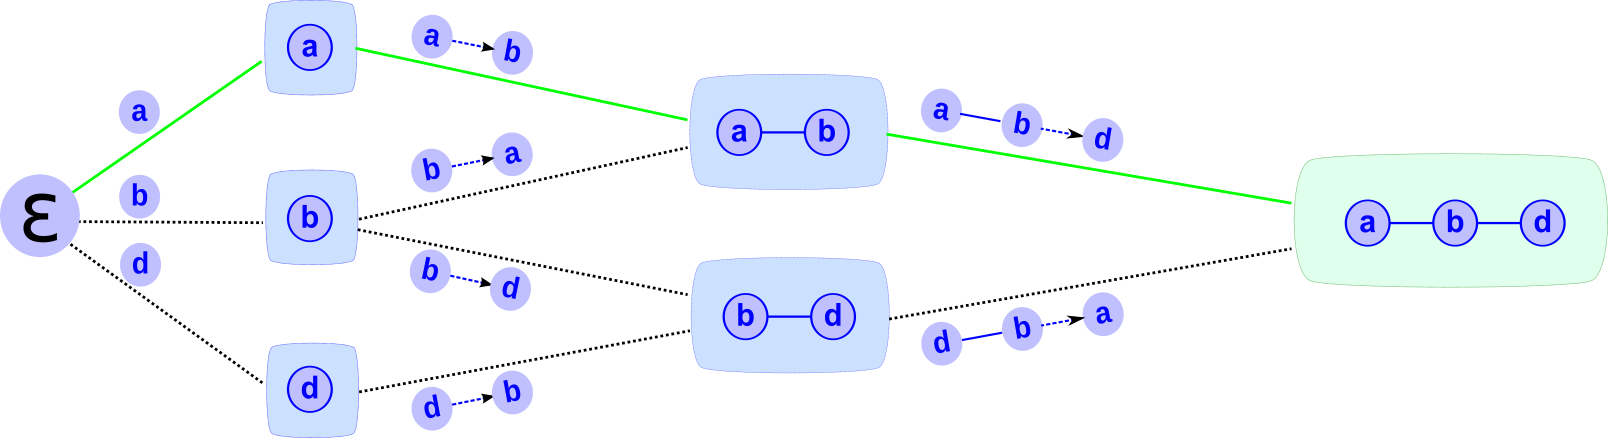
\includegraphics[width=300px]{Figures/s2m/indexation/glouton.png}
  \caption{\label{glouton}En vert le chemin prit par l'algorithme glouton pour générer la chaîne du motif a-b-d}
\end{figure}

\subsubsection{Indexation Markovienne}

\paragraph{}En utilisant la méthode gloutonne, nous obtenons rapidement les chaînes de tous les motifs que nous
souhaitons indexer. Cependant, dans certains cas, une chaîne générée de cette manière peut ne pas du tout être optimale.
Dès le tout début de la chaîne il est possible que l'algorithme fasse des choix optimaux localement qui vont ensuite mener à un
enlisement global. Nous allons nous appuyer sur les figures \ref{apprentissage} et \ref{glouton} pour monter que même sur un si
petit exemple l'algorithme glouton n'a pas choisi le meilleur chemin.

\paragraph{}Afin d'évaluer la qualité d'une chaîne, nous allons calculer son temps d'exécution sur notre base d'apprentissage.
Partons de la définition d'une chaîne : Une chaîne est composée d'une succession de noeuds. Ces noeuds vont lors de l'isomorphisme
être recherchés dans l'ordre. Pour rechercher une chaîne de taille $n$ ($c_n$), il faut donc $n$ extensions successives. On
peut donc écrire que le temps de recherche d'une chaîne est le temps cumulé de recherche de ses extensions :

\begin{equation}
 T(c_n) = T(p_0 \rightarrow p_1 \rightarrow ... \rightarrow p_n) = \sum_{i=1}^n T(p_{i-1} \rightarrow cp_i)
\end{equation}

Où $T()$ est la fonction représentant le temps de recherche d'une chaîne, $p_i$ le un motif de taille $i$ et $p_{i-1} \rightarrow
p_i$ la dernière extension d'une chaîne $c_i$ représentée par le passage du motif $p_{i-1}$ au motif $p_i$. Il est à noter que
rechercher une chaîne de taille 1 revient à étendre un motif vide. C'est à dire qu'il est nécessaire de parcourir l'intégralité
des noeuds de la cible dans laquelle on recherche le motif et ce quel que soit le motif. Sur notre base d'apprentissage il faudra
donc tester tous les noeuds de tous les peptides d'apprentissage pour la première extension.

\begin{figure}
  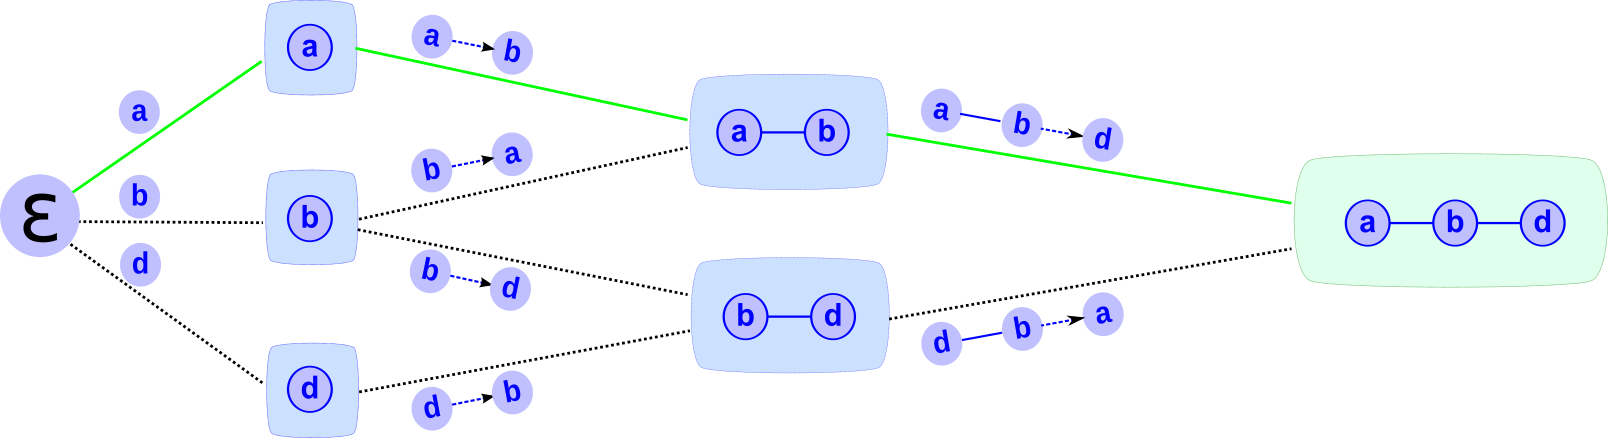
\includegraphics[width=300px]{Figures/s2m/indexation/glouton.png}
  \caption{\label{arite}Arité restante pour les différents noeuds d'un graphe chimique simple}
\end{figure}

\paragraph{}Lors d'une recherche d'une chaîne $c_{n-1}$, il est possible de trouver isomorphismes sur la cible
(potentiellement partiellement recouvrant). Afin calculer le temps de recherche de $c_n$ nous devons prendre en compte
la quantité de sous isomorphismes précédemment trouvés. Le calcul du temps de recherche de $c_n$ correspondra donc au temps de
calcul de $C_{n-1}$ auquel on vient ajouter le temps de recherche de la dernière extension sur chacun des isomorphismes de taille
$n-1$. Il faut également tenir compte du nombre d'extensions qui vont être essayées. Par exemple, si l'on cherche à étendre un
isomorphisme précédent en suivant un lien qui est enraciné sur un $NH$, il ne reste qu'une liaison à explorer (le $N$ ayant déjà
une liaison avec son $H$ et une liaison avec le reste du motif déjà recherché). En reprenant la même logique pour un $C$, il
resterait donc trois liaisons à suivre. Nous appellerons cette quantité l'arité restante. On peut donc écrire :

\begin{equation}
 T(p_{n-1} \rightarrow p_n) = n_{p_{n-1}} \times a_{p_{n-1} \rightarrow p_n} \times t
\end{equation}

Où $n_{p_{n-1}}$ est le nombre d'isomorphismes trouvés pour le motif $p_{n-1}$, $a_{p_{n-1} \rightarrow p_n}$ est l'arité restante
de l'atome depuis lequel on étend le motif $p_{n-1}$ vers le motif $p_n$ et $t$ le temps nécessaire pour une comparaison de deux
labels (ce temps peut être considéré constant)

\paragraph{}Combinons les deux équations précédentes, pour obtenir une formule globale :

\begin{equation}
 T(c_n) \propto^t N + \sum_{i=2}^n (n_{p_{i-1}} \times a_{p_{i-1} \rightarrow p_i})
\end{equation}

\begin{figure}
  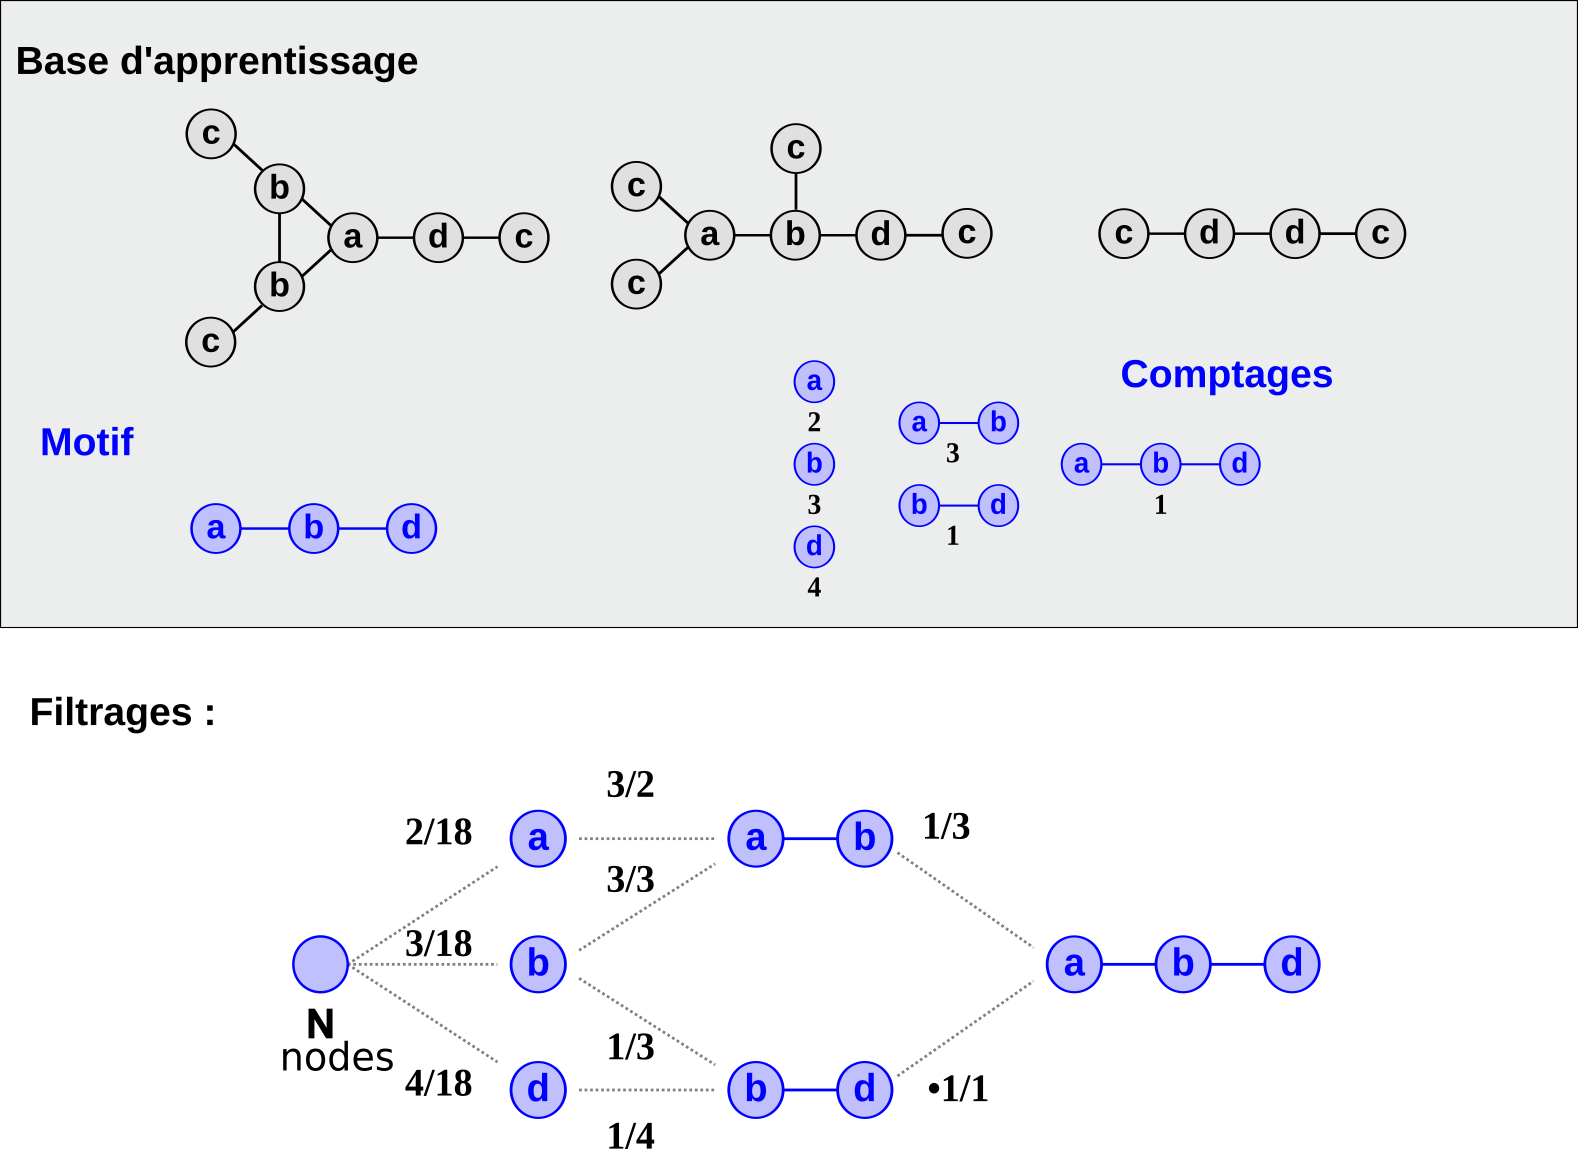
\includegraphics[width=300px]{Figures/s2m/indexation/apprentissage_comptage.png}
  \caption{\label{app_compt}Base d'apprentissage accompagnée des comptages de tous les $n_{p_{n}}$}
\end{figure}

\paragraph{}En utilisant les comptages fait sur la base d'apprentissage (Voir \ref{app_compt}) ainsi que le calcul de l'arité
restante de chaque noeud à chaque étape, nous allons pouvoir estimer sur la base, un temps d'exécution de la recherche d'une
chaîne. Ce temps est un coût exact de le recherche sur la base d'apprentissage. En normalisant cette valeur par le nombre de
noeuds de la base nous pouvons obtenir le coût de recherche par noeud et ainsi pouvoir estimer le temps de calcul quelque soit
la taille de la ou les molécules à analyser.

\begin{equation}
 T(c_n) \propto^t 1 + \sum_{i=2}^n ({n_{p_{i-1}} \over N} \times a_{p_{i-1} \rightarrow p_i})
\end{equation}

\paragraph{}Redéfinissons la notation ${n_{p_{i-1}} \over N}$ qui correspond à un taux de filtrage d'un motif de taille $i-1$.
Appelons ce taux $F_{i-1}$. Cette notation peut à son tour être transformée en
produit des filtrages de chaque extension d'une chaîne. Les valeurs des filtrages estimés s'obtiennent immédiatement à partir des
comptages dans la base d'apprentissage (Voir \ref{app_compt} pour un exemple). NB : Le taux de filtrage peut être supérieur à 1
car il est possible d'obtenir plus d'isomorphismes après une extension que avant.

\begin{equation}
 {n_{p_{i-1}} \over N} = F_{i-1} = \prod_{i=0}^{i-1} f_i
\end{equation}

\begin{equation}
 T(c_n) \propto^t 1 + \sum_{i=2}^n a_{p_{i-1} \rightarrow p_i} \prod_{j=0}^{i-1} f_j
\end{equation}

\paragraph{}Le temps de recherche optimal d'un motif est donc le temps de recherche de la chaîne qui minimise le coût. Donc :

\begin{equation}
 T(p_n) = \min c_n, \forall c_n
\end{equation}


\paragraph{}Appliquons maintenant cette formule de calcul du temps sur notre exemple pour trouver la meilleure chaîne possible par
rapport à la base d'apprentissage. Pour le motif de l'exemple, nous pouvons nommer les différentes chaînes possibles de $\alpha$
jusque $\delta$.

\[
\begin{array}{ccccccc}
 c         & = & p_1 & \rightarrow & p_2     & \rightarrow & p_3 \\
 c_\alpha  & = & a   & \rightarrow & a\!-\!b & \rightarrow & a\!-\!b\!-\!d \\
 c_\beta   & = & b   & \rightarrow & a\!-\!b & \rightarrow & a\!-\!b\!-\!d \\
 c_\gamma  & = & b   & \rightarrow & b\!-\!d & \rightarrow & a\!-\!b\!-\!d \\
 c_\delta  & = & d   & \rightarrow & b\!-\!d & \rightarrow & a\!-\!b\!-\!d \\
\end{array}
\]

Naïvement, on peut appliquer la formule sur chacune des chaînes possible et trouver la chaîne optimale qui minimise la fonction de
coût. Développons l'exemple pour la chaîne $c_{\alpha}$.

\[
\arraycolsep=1.4pt\def\arraystretch{1.2}
\begin{array}{cccccccccccccc}
  c_\alpha    & =  & \epsilon &  \rightarrow &  \multicolumn{3}{c}{a} & \rightarrow & \multicolumn{3}{c}{a\!-\!b} &  \rightarrow & \multicolumn{1}{c}{a\!-\!b\!-\!d} &\\
  T(c_\alpha)   & =  & T( \epsilon &  \rightarrow &  a)  & + & T( a &  \rightarrow  & a\!-\!b) & + & T(a\!-\!b &  \rightarrow & a\!-\!b\!-\!d) &\\
                    & \propto_{N}  &  \multicolumn{3}{c}{1} &  + & \multicolumn{3}{c}{3 \times \frac{2}{18}} & + & \multicolumn{3}{c}{  (3-1)\times \frac{2}{18} \times \frac{3}{2}} &\\
                    & = &  \multicolumn{3}{c}{1} &  + & \multicolumn{3}{c}{\frac{1}{3}} & + & \multicolumn{3}{c}{\frac{1}{3}}   & \quad= \quad\frac{5}{3} \\

\end{array}
\]

\paragraph{}En appliquant cette formule sur toutes les chaînes on peut se rendre compte que certains de nos calculs sont inutiles.
Prenons l'exemple des chaînes $c_{\alpha}$ et $c_{\beta}$. Le dernier calcul de la chaîne $c_{\beta}$ est inutile. Lors
du calcul des deux chaînes, on aurait pu se rendre compte que l'on pouvais déjà décider de quelle chaîne était la meilleure à
partir du résultat de la sous chaîne $a-b$. Ceci nous amène à transformer le calcul sous forme de programmation dynamique dont les
formules de récurrence sont les suivantes.


\begin{equation}
 T(\epsilon \rightarrow p_1) = 1
\end{equation}
\begin{equation}
 T(p_n) = \min^{p'_{n-1} \subset p_n} (T(p'_{n-1}) + T(p'_{n-1} \rightarrow p_n))
\end{equation}

Où la fonction de minimisation s'applique sur l'ensemble des $p'_{n-1}$ et $p'_{n-1}$ est un motif connexe de taille $n-1$ inclus
dans $p_n$. Pour la recherche de motif dans l'exemple on obtient le chemin $c_{\delta}$ minimisant le coût. On peut voir le
détail de la recherche de ce motif sur la figure \ref{markov}.

\begin{figure}
  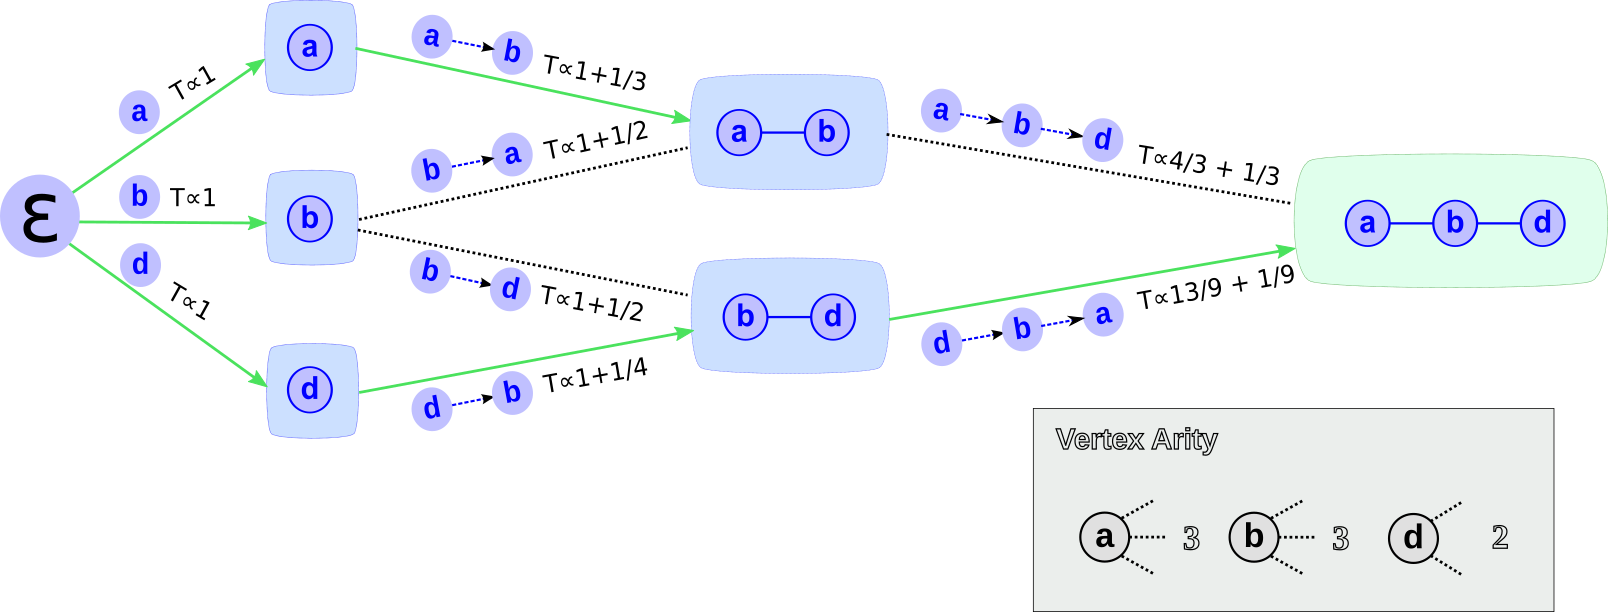
\includegraphics[width=300px]{Figures/s2m/indexation/markov.png}
  \caption{\label{markov}En vert le chemin prit par l'algorithme markovien pour générer la chaîne du motif a-b-d}
\end{figure}

\paragraph{}Cette méthode exacte nous permet de garantir la qualité de nos chaînes sur la base d'apprentissage mais cela se paye
en temps de calcul. En effet, même par programmation dynamique le temps de pré-calcul des chaînes est très élevé si les motifs sont
composés de nombreux branchements et d'une grande diversité de noeuds. Calculons la complexité en considérant que chacun des
labels soit différent (C'est ce que nous avons essayer de faire pour simplifier la recherche d'isomorphismes).

Une chaîne (au sens ligne et pas chaîne comme défini ici) représente le motif le plus simple. Pour une chaîne de noeuds de taille 
$n$, on peut trouver un motif de taille $n$ puis deux de taille $n-1$ puis 3 de taille $n-2$, ... Pour calculer le coût du motif
de taille $n$ il nous faut calculer récursivement tous les motifs de taille inférieure. Dans le meilleur des cas la programmation
dynamique sera donc de complexité de l'ordre de $n^2$.

Le pire motif qui peut être défini est une clique. Dans le cas d'une clique de taille $n$ pour calculer le coût du motif il faudra
calculer $n-1$ parmi $n$ valeurs puis $n-2$ parmi $n$, ... Dans ce cas, la complexité sera de l'ordre de $2^n$.

La redondance des labels permet quant à elle de couper certaines branches lors de l'indexation et permet ainsi de diminuer un peu
la complexité. Cependant, l'ordre de grandeur n'en est pas modifié.

\begin{equation}
 Cplx_{chaine} = n + n-1 + ... + 2 + 1 = \sum_{i=1}^n i = {{n (n+1)} \over 2} = O(n^2)
\end{equation}
\begin{equation}
 Cplx_{clique} = {n \choose n} + {n \choose n-1} + ... + {n \choose 2} + {n \choose 1} = \sum_{k=1}^n {n \choose k} = O(2^n)
\end{equation}


\subsubsection{Indexation hybride}

\paragraph{}Dans un exemple précédent (TODO : ref), nous avons montré que le début d'une chaîne est très critique pour le temps
de recherche de celle-ci. L'idée est donc de générer la chaîne par un mélange des deux techniques précédentes. Les débuts de la 
chaîne seront être recherchés en exact jusqu'à une taille $k$ définie à l'avance puis le reste des extensions se feront en
utilisant l'algorithme glouton. Cette découpe des chaînes en deux parties nous permet de garantir une recherche très rapide d'un
motif sur la base d'apprentissage tout en limitant fortement le temps de pré-calcul nécessaire pour la construction de l'index.



\subsection{Des monomères aux résidus}


\subsubsection{Résidus}

\paragraph{}L'algorithme et les indexes présentés dans la section précédente permettent de retrouver rapidement toutes les
occurrences d'un motif au sein d'une molécule cible. Jusqu'à présent nous avons laissé supposé que dans notre cas
nous recherchions des monomères dans des peptides. Ceci n'est en fait pas applicable directement. En effet, on ne retrouve jamais
un monomère en entier au sein d'un polymère. Lorsque les monomères sont liés ensemble pour former le polymère, chacun perd une
partie de ses atomes dans ces liaisons. Nous appellerons les molécules incluses des résidus (les monomères sans leurs atomes de
liaison).

\paragraph{}Prenons l'exemple de la Cystéine pour bien comprendre (Voir figure \ref{cys_ex}).
La cystéine est présente dans 47 peptides de la base de données
NORINE. Dans certains peptides comme ACV, la cystéine est incluse en effectuant deux liaisons peptidiques avec ses voisins. D'un
côté elle perd les atomes $OH$ de son groupement $COOH$ pour aller se lier à un groupe $NH_2$ qui perd un de ses $H$. Le tout
libère un $H_2O$ pendant la réaction. De l'autre côté elle perd un $H$ de son groupement $NH_2$ pour effectuer la même opération
inversée. Au total la cystéine présente dans ce peptide a donc perdu trois atomes sur deux sites distincts. Dans d'autre cas
comme dans la malformin A1, la cystéine effectue une troisième liaison au niveau de son atome de soufre en perdant un atome 
d'hydrogène pour se lier avec un autre atome de soufre et ainsi réaliser un pont disulfure. Sur ce simple exemple on remarque que
non seulement le monomère n'est jamais inclus en entier mais en plus, il peut être inclus dans un polymère de plusieurs manières
différentes. Il est donc nécessaire de connaître les différents résidus possibles pour chaque monomère afin de pouvoir les
rechercher en utilisant l'algorithme de recherche exact décrit précédemment.

\begin{figure}
  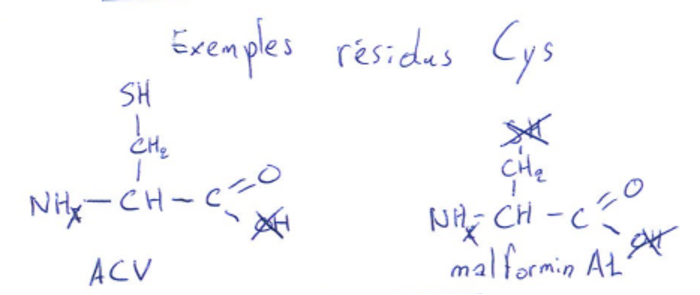
\includegraphics[width=300px]{Figures/s2m/residues/cys_exemple.pdf}
  \caption{\label{cys_ex}Deux résidus différents présents dans deux peptides différents tout deux obtenus à partir de la Cystéine}
\end{figure}


\subsubsection{Familles de résidus}

\paragraph{}Différents résidus d'un même monomère peuvent être créés selon les contextes. Pour connaître les différents résidus
possibles pour chaque monomère nous devons donc connaître les règles qui régissent les liaisons. Par exemple pour la liaison
peptidique précédemment citée, nous pouvons déduire deux règles. Si un $COOH$ est détecté alors le monomère peut potentiellement
perdre son $OH$. De la même manière pour la seconde moitié de la liaison on peut perdre un $H$ pour un $NH_2$ détecté. En
regardant précisément les liaisons qui apparaissent pour un type de polymère, nous pouvons créer une liste de règles de perte
d'atomes. En appliquant ses règles récursivement sur un monomère, nous pouvons générer tous ses résidus candidats. Notons que
certaines règles comme celles du pont disulfure décrite précédemment, ne s'applique qu'en présence d'une autre liaison. Il n'est
donc jamais nécessaire de générer le résidu qui contient uniquement cette liaison. Ici nous n'aurons donc jamais de résidus
uniquement constituée d'une liaison sulfure. Il est
à noter que moins une règle sera précise et plus le nombre de résidus générés sera important. Imaginons une règle qui nous dirait
dans un cadre de chimie organique que pour tout carbone étant lié à au moins un hydrogène, l'atome d'hydrogène peut être perdu
pour former une liaison. Si $n$ est le nombre d'atomes de carbone dans la molécule ($n$ représente une grande proportion d'atomes
dans une molécule organique), alors on peut générer un nombre de résidus de l'ordre de $n^2$.

\begin{figure}
  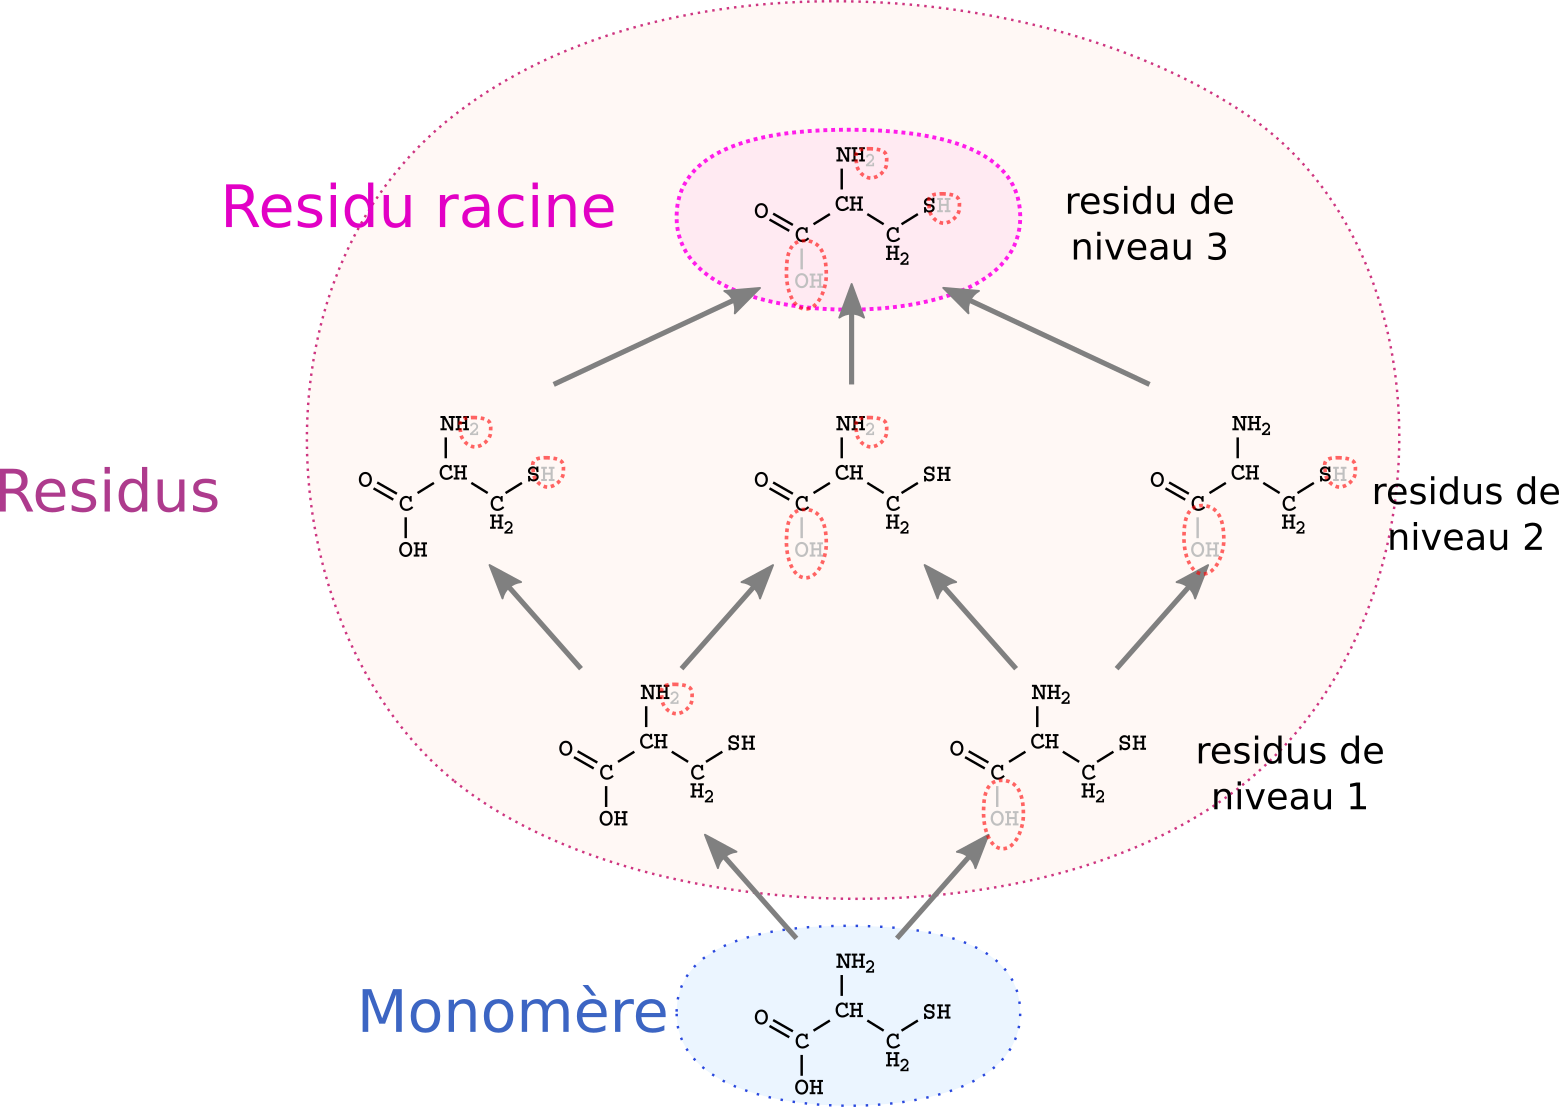
\includegraphics[width=300px]{Figures/s2m/residues/cystein_family.png}
  \caption{\label{sulfure}Représentation de la famille des résidus de la cystéine}
\end{figure}

\paragraph{}Comme présenté dans la figure \ref{sulfure}, les différents résidus générés peuvent être représentés sous la forme
d'un Graphe Orienté Acyclique (GOA). Le monomère de base ainsi que chacun des résidus est un noeud du graphe et chaque arc est un
lien de parenté entre noeuds. Un arc sera par exemple créé entre un résidu auquel on a appliqué une seule règle et le monomère.
Nous appellerons \textbf{famille} cette représentation des résidus sous forme de GOA.

\paragraph{}Le noeud le plus éloigné du monomère sera le noeud
qui aura subit le plus de modification. Nous appellerons le résidu de ce noeud le \textbf{résidu racine}. Ce résidu à un intérêt
tout particulier pour la recherche du monomère. En effet, si le résidu racine n'est pas trouvé alors qu'il est celui
qui possède le moins d'atomes dans la famille, cela veut dire qu'aucun membre de la famille ne pourra être trouvé. On peut même
aller plus loin en étendant le raisonnement à tous les résidus. Si un résidu de niveau $n$ n'est pas trouvé alors il est inutile
de rechercher ses résidus parents de niveau $n-1$. Il est également vrai de dire qu'il est inutile de chercher un résidu parent de
niveau $n-1$ si tout ses enfants de niveau $n$ n'ont pas été trouvés.

\paragraph{}En connaissant la structure familiale des résidus ainsi qu'un ordre naturel de recherche pour passer d'un résidu à
l'autre, nous pouvons déduire une structure globale de recherche. Découle donc de cette structure familiale un ordre de recherche
naturel depuis le résidu racine jusqu'aux résidus de niveau 1 (Inutile de rechercher le monomère car il n'étant jamais inclus tel
quel). De plus, il n'est jamais nécessaire de
recalculer complètement un isomorphisme une fois que la racine trouvée. Pour passer d'un résidu $r$ à l'un de ses parents $p$ il
suffit de rechercher à étendre l'isomorphisme de $r$ avec les atomes que nous avions considérés perdus pour passer de $p$ à $r$
lors de la construction de la famille. De plus, le fait de ne pas tout recalculer à chaque étape nous permet de ne calculer
l'index que pour les résidus racine. Le reste des résidus n'est indexé que sur les extensions a effectuer depuis leurs enfants.
L'algorithme qui décrit la recherche d'une famille est donc le suivant :

\paragraph{}
\begin{algorithm}[H]
  \caption{Algorithme de recherche des résidus d'une famille}
  \KwData{Un graphe $G(V, E)$ représentant le polymère cible et une famille $F_m$ de résidus pour le monomère $m$. Le résidu $r_r$
  étant le résidu racine de la famille.}
  \KwResult{Un ensemble de tuples constitués d'un résidu et d'un ensemble de position. Ces tuples représentent chacun un
  isomorphisme du résidu avec une sous partie du polymère.}
  Soit $S$ un ensemble de tuples solution initialement vide\;
  $S \gets subgraphIsomorphism (G, r_r)$\;
  
  \If {$S$ est vide} {
    \KwRet $S$\;
  }
  
  Soit $P$ un ensemble de résidus à procésser initialisé avec les parents de $r_r$\;
  \While {$P$ n'est pas vide} {
    $r \gets supprimeUnElement(P)$\;
    $Tmp \gets subgraphIsomorphism (G, r)$\;
    
    \If {$Tmp$ n'est pas vide} {
      Ajouter $Tmp$ dans $S$\;
      \For{$p \subset parents(r)$}{
	\If {Tous les enfants de $p$ ont été trouvés} {
	  Ajouter $p$ dans $P$\;
	}
      }
    }
  }
  
  \KwRet $S$;
\end{algorithm}




\subsection{Pavage de monomères}

\subsubsection{Pavage : définition}

\paragraph{}La méthode de recherche des isomorphismes de sous graphe présentée précédemment, nous permet de trouver
toutes les occurrences de chacun des monomères dans un peptide cible.

Puisque nous connaissons les atomes contenus dans chacun des isomorphismes découverts, nous pouvons également connaître chacun des
isomorphismes découvert par atome.
L'étape de pavage consiste à choisir un sous ensemble des isomorphismes trouvés, de manière à maximiser les atomes couverts par ces
isomorphismes en ayant pour chaque atome au plus un seul isomorphisme présent dans ce sous ensemble.

Faisons une analogie avec un puzzle. La phase d'isomorphisme nous permet d'obtenir de nombreuses pièces de puzzle. Ces pièces ne
permettent pas forcément de reconstituer un puzzle complet. De plus, parmi les pièces que nous disposons, certaines se
chevauchent. La phase de pavage consiste à choisir parmi les pièces celles que l'on souhaite garder en maximisant le
remplissage de notre puzzle et sans avoir de pièces chevauchantes (figure \ref{puzzle}).

\begin{figure}
  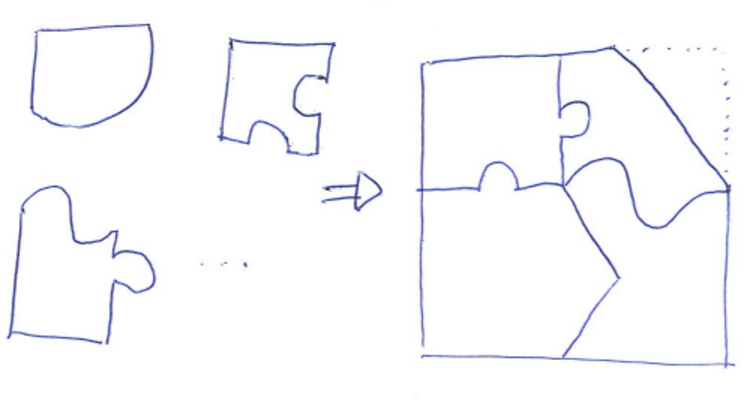
\includegraphics[width=300px]{Figures/s2m/pavage/puzzle.pdf}
  \caption{\label{puzzle}Un pavage est une recherche des meilleures pièces permettant de construire le puzzle des monomères}
\end{figure}

\paragraph{}Dans l'idéal, toutes les pièces nécessaire à la reconstruction du puzzle complet sont présentes dans l'ensemble des
pièces trouvées. Dans le cas contraire, on ne peut pas reconstruire complètement le peptide à partir des résidus trouvés. 
Dans ce cas, notre
but sera alors de trouver un assemblage le plus complet possible. Si beaucoup de résidus ont été trouvés lors de la première phase
il est également possible que nous ne trouvions pas qu'une seule solution de reconstruction. Nous n'aurons alors aucun moyen
purement algorithmique de choisir quelle est la meilleure façon de découper ces peptides.

\begin{figure}
  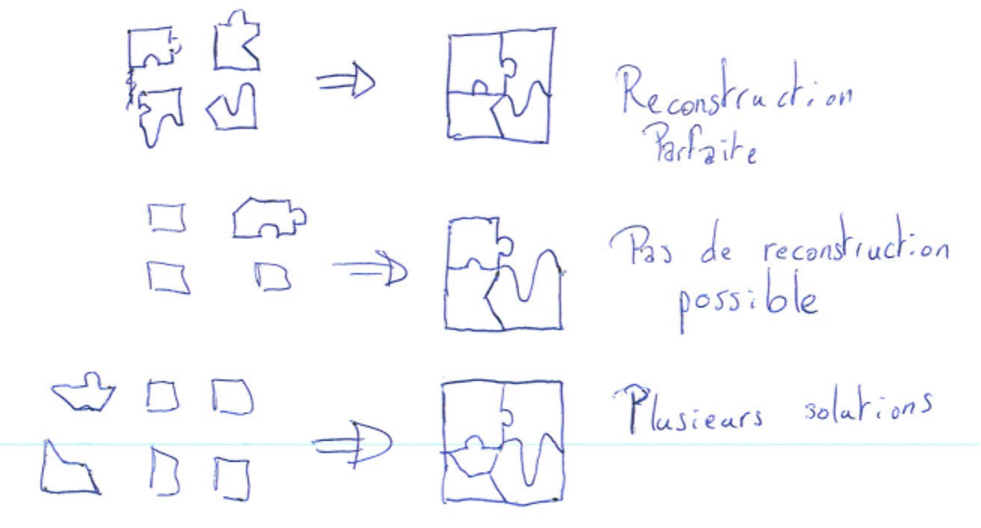
\includegraphics[width=300px]{Figures/s2m/pavage/reconstructions.pdf}
  \caption{\label{reconstruction}Les différents types de reconstruction que l'on peut obtenir par le pavage}
\end{figure}




\subsubsection{Pavage exact par optimisation linéaire}

\begin{figure}
  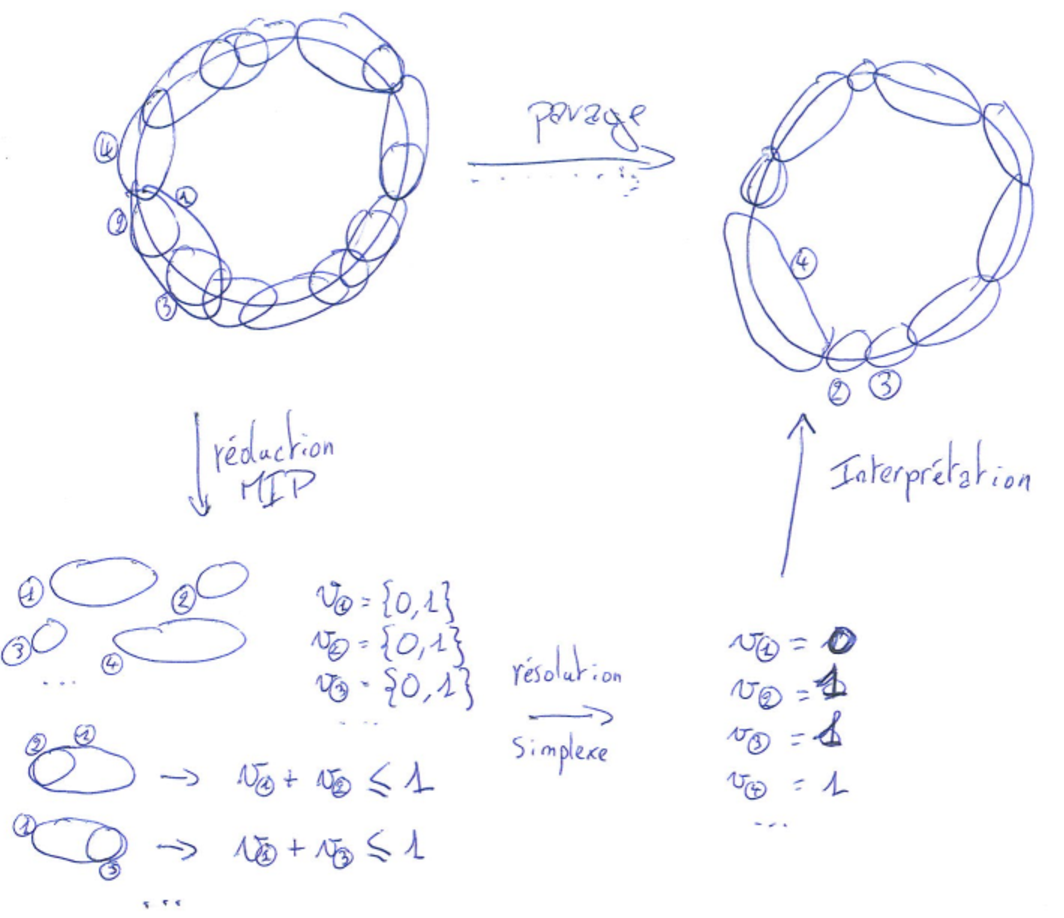
\includegraphics[width=300px]{Figures/s2m/pavage/reduction.pdf}
  \caption{\label{reduction}Représentation globale de la réduction du problème de pavage en MIP puis reconstruction de la
  solution}
\end{figure}

\paragraph{}Nous allons ici résoudre le problème de pavage en exact par utilisation de la programmation linéaire (LP). Un
problème de programmation linéaire est un
problème représenté par un ensemble de variables, une fonction de score ainsi qu'une liste de contraintes sur les variables. La
fonction de score est accompagnée d'un objectif de maximisation ou de minimisation. Ce type de problème est classiquement résolu
par l'algorithme du simplexe\cite{murty_linear_1983}. Depuis la publication, de nombreuses variante de l'algorithme ont été
créées. L'une d'elle, appelée ``Mixed Integer Programming'' (MIP)\cite{wolsey_mixed_2007}, permet de résoudre des problèmes
pour lesquels les variables sont des entiers.

\paragraph{}Dans notre cas, nous allons rechercher les résidus qui seront utiles pour notre assemblage final.
Ainsi nous représentons la présence ou l'absence dans la solution finale d'un résidu trouvé durant la première phase par une
variable binaire (0 pour l'absence et 1 pour la présence).

\begin{equation}
 \forall r_i \exists v_{r_i}, v_{r_i} \in \{0, 1\}
\end{equation}

Où $r_i$ représente le i-ème résidu et $v_{r_i}$ la variable binaire correspondant à $r_i$.

\paragraph{}Nous souhaitons également interdire la possibilité de chevauchement de deux résidus. Nous pouvons caractériser cela
par la restriction d'avoir au plus un résidu présent sur chaque atome (ie une variable avec la valeur 1). On obtient donc une
contrainte pour chaque atome ; ces contraintes étant
représentées par le fait que la somme de toutes les variables des résidus présents sur un atome ne peut être supérieure à 1.

\begin{equation}
 c_a : \sum^{r_i} v_{r_i} \leqslant 1, a \in r_i
\end{equation}

Où $a$ est l'atome correspondant à la contrainte $C_a$.

\paragraph{}Enfin, nous cherchons à maximiser le nombre d'atomes couverts par les résidus présents. La fonction de score sera
donc la somme des présences des résidus pondérée par la taille de chaque résidu :

\begin{equation}
 score : \sum^{r_i} v_{r_i} * size(r_i)
\end{equation}

\paragraph{}La réduction de notre problème de pavage en un MIP nous permet d'utiliser des solveurs déjà existant pour trouver la
solution exacte. Nous pouvons par exemple utiliser la bibliothèque GLPK (l'une des seules bibliothèques de LP sous licence libre).

\paragraph{Schéma : Vue globale de la réduction en MIP}

\paragraph{}Bien que cette solution soit élégante, MIP dans sa version ne contenant que des variables binaires fait partie des 21
problèmes NP-complets de Karp\cite{karp_reducibility_1972}. Il n'existe donc actuellement aucune méthode ne permettant de
résoudre ce problème en temps polynomial. Pour les cas les plus difficiles, il est donc nécessaire de trouver un moyen plus
rapide d'obtenir une solution.

\paragraph{Stackexchange ?} Preuve NP complétude ?
http://cs.stackexchange.com/questions/48775/np-hardness-of-covering-with-rectangular-pieces-google-hash-code-2015-test-roun/49074





\subsubsection{Pavage glouton}

\paragraph{}L'un des moyen d'obtenir très rapidement une solution est de trier les résidus dans un ordre voulu puis de parcourir
la liste triée en ajoutant le résidu courant à la solution uniquement si il ne chevauche aucun autre résidu de la solution.
On pourra toujours trouver au moins un tri de la liste permettant d'atteindre la solution optimale. En faisant cela on reporte la
difficulté du problème sur les critères de tri de la liste mais on garantit une très grande rapidité d'exécution.

\paragraph{}
\begin{algorithm}[H]
  \caption{Algorithme de pavage glouton}
  \KwData{Un peptide requête $P$ et une liste de résidus $RES$ mappés sur $P$ lors de la phase d'isomorphisme}
  \KwResult{Un sous-ensemble de $RES$ de pièces non chevauchantes sélectionnées par l'algorithme glouton.}
  Soit $SOL$ un ensemble solution de résidus, initialement vide\;
  
  Trier $RES$ selon les critères gloutons\;
  \For {$r_i \in RES$} {
    \If {$r_i$ ne chevauche aucun $r_j$ tq $r_j \in SOL$} {
      Ajouter $r_i$ à $SOL$\;
    }
  }
  
  \KwRet $SOL$;
\end{algorithm}

\paragraph{}Cet algorithme nécessite un tri sur une liste de $n$ résidus ($O(n log n)$) puis consomme ensuite un élément de la
liste à chaque tour de boucle ($O(n)$). Contrairement à la résolution exacte présentée ci-dessus, si la fonction de comparaison
pour le tri ne dépendent pas de $n$ cet algorithme est polynomial.
Nous pouvons donc garantir la rapidité d'exécution à partir du moment où nous choisissons des critères de tri simples.

\paragraph{}Le but est d'opter pour l'efficacité maximale locale en espérant que l'efficacité globale sera également maximale.
Dans notre cas, la probabilité de trouver par hasard un résidu dans un peptide est
inversement proportionnelle au nombre d'atomes qu'il contient (La composition intervient également mais nous cherchons ici des
critères simples). On peut donc dire qu'un résidu est d'autant plus ``efficace'' que sa probabilité d'apparition par hasard est
faible. Le premier critère consiste donc à trier les résidus par taille décroissante (nombre d'atomes dont hydrogènes).
C'est un critère classiquement utilisé pour la résolution gloutonne du problème du sac à dos\cite{_probleme_2016}.

\begin{figure}
  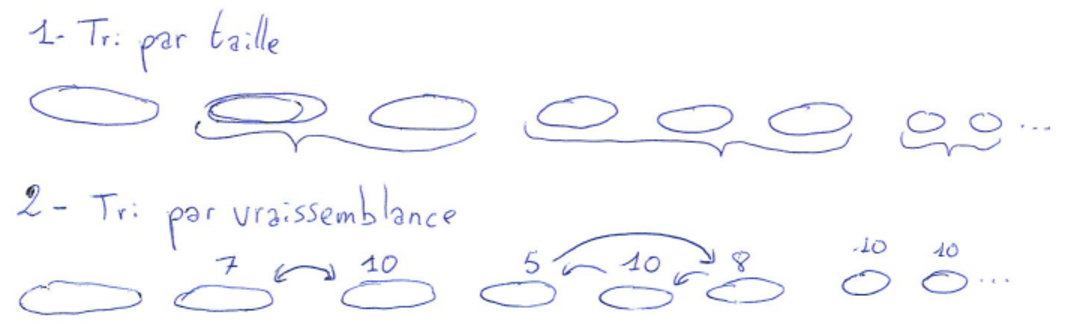
\includegraphics[width=300px]{Figures/s2m/pavage/tri_glouton.pdf}
  \caption{\label{glouton}En vert le chemin prit par l'algorithme glouton pour générer la chaîne du motif a-b-d}
\end{figure}

\paragraph{}Lorsque les résidus sont issus de monomères très similaires en taille, il arrive fréquemment que nombre d'entre eux
aient exactement le même nombre d'atome.
Dans ce cas, le critère de taille n'est plus suffisant pour le tri et il nous faut en ajouter d'autres.

En plus de leur taille les résidus peuvent être caractérisés par leurs types de liaisons.
Chaque résidu forme des liens qui peuvent être différent d'un résidu à l'autre.
Certains liens apparaissent fréquemment alors que d'autres beaucoup moins, ce qui nous permet en théorie d'estimer les
probabilités d'apparition d'un lien par rapport à un autre.
Ainsi, on peut considérer qu'un résidu contenant des liens qui apparaissent très souvent a plus de chance d'être le bon résidu
face à un second de même taille contenant des liens moins fréquents.
Cependant, nous ne possédons pas de statistiques sur les fréquences d'apparition des types de lien.
Pour tout même pouvoir classer les résidus de cette manière, nous requérons l'expertise de l'utilisateur.

Avant la phase d'indexation, l'utilisateur doit définir les différentes
règles de liaison qu'il veut voir apparaître dans les monomères. C'est à ce moment que nous lui demandons également de remplir
une valeur pour chacune de ces règles. Cette valeur représente le poids que l'utilisateur souhaite donner à chacune des liaisons
possibles. Ce poids représente la confiance que l'on donne à l'apparition d'un type de liaison. En s'appuyant sur cette
information, nous
sommes capable pour chaque résidu de donner un poids moyen par liaison et ainsi de comparer la confiance que l'on peut
avoir en chacun des résidus. Les résidus de poids moyen les plus élevés seront triés au début de la liste.

\paragraph{}Dans le cas où plusieurs résidus ne peuvent être départager lors du tri, nous considérons qu'ils sont équivalents et
leur ordre sera aléatoire.


\subsubsection{Modulation de pavage}

\paragraph{}Le pavage glouton est un très bon compromis de rapidité mais il ne garantit pas la qualité du résultat.
Sur certaines données, alors que la phase d'isomorphisme a identifié tous les monomères qui sont effectivement présents dans le
peptide, le pavage correct n'est pas trouvé, l'algorithme nous laissant avec une solution partielle.
Lorsque qu'un cas de pavage incomplet se présente, nous pouvons donc nous demander si il ne serait pas possible de tout de même
obtenir la solution avec les isomorphismes déjà effectués.
Nous proposons de repartir de la solution partielle et de chercher intelligemment dans son voisinage afin de nous convaincre qu'il
n'est pas possible de faire mieux.

\paragraph{}L'algorithme de modulation que nous allons vous présenter permet d'être certain de passer par la meilleure solution si
elle existe.
De plus, n s'appuyant sur les critères de l'algorithme glouton nous essayons de rapidement trouver cette solution.
Nous allons regarder au sein de la liste triée des résidus afin d'ajouter à la solution le premier résidu couvrant au moins un
atome non couvert dans la solution partielle.
Puisque ce résidu n'a pas été choisi lors du pavage, il chevauchera au moins un résidu existant dans la solution.
Pour obtenir une solution viable, nous enlevons les résidus chevauchés de la solution en interdisant de les remettre (les enlever
pour les remettre ne serait pas productif) puis nous essayons de compléter la solution en relançant un pavage.
Si la solution n'est pas complète, nous pouvons relancer la procédure récursivement.
La récursion se termine soit lorsqu'une solution complète est trouvée soit lorsqu'il n'est plus possible de choisir de résidus
couvrant des zones non couvertes de la solution partielle.

\begin{figure}
  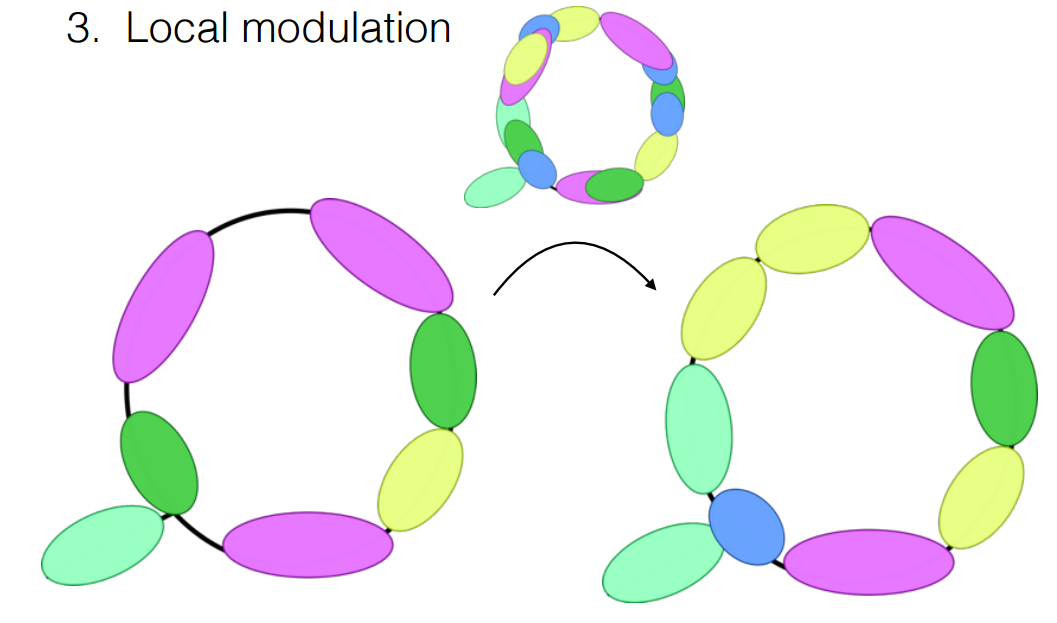
\includegraphics[width=300px]{Figures/s2m/pavage/modulation.png}
  \caption{\label{glouton}En vert le chemin prit par l'algorithme glouton pour générer la chaîne du motif a-b-d}
\end{figure}

\paragraph{}
\begin{algorithm}[H]
  \caption{Algorithme de modulation du pavage}
  \KwData{Un peptide requête $P$ et une liste de résidus $RES$ mappés sur $P$ lors de la phase d'isomorphisme et triés par
  l'algorithme glouton, une pré-solution $SOL$ et un ensemble $INT$ de résidus interdits d'utilisation.}
  \KwResult{$SOL$, un sous-ensemble de $RES$ de pièces non chevauchantes sélectionnées par la modulation}
  
  $r \gets$ Premier élément de $RES$ couvrant au moins un atome non couvert et n'étant pas présent dans $INT$\;
  \If {$r$ n'existe pas} {
    \KwRet Impossible\;
  }
  Soit $SUPPR$ une liste de résidus\;
  \For {$r_i \in SOL$} {
    \If {$r_i$ chevauche $r$} {
      Ajouter $r_i$ à $SUPPR$\;
      Supprimer $r_i$ de $SOL$\;
      Ajouter $r_i$ à $INT$\;
    }
  }
  
  Lancer un pavage pour compléter $SOL$\;
  
  \If {$SOL$ couvre $P$ à 100\%} {
    \KwRet $SOL$\;
  }
  
  $SOL \gets$ Modulation récursive\;
  
  \If {$SOL = $ Impossible} {
    Supprimer $r$ de $SOL$\;
    Ajouter $r$ dans $INT$\;
    \For {$r_i \in SUPPR$} {
      Enlever $r_i$ de $INT$\;
      Ajouter $r_i$ à $SOL$\;
    }
  }
  
  \KwRet $SOL$\;
\end{algorithm}


\paragraph{}L'algorithme permet d'explorer toutes les solutions possibles jusqu'à obtenir la meilleure. Le problème majeur
est que si une solution parfaite n'existe pas, l'algorithme de modulation va parcourir tout l'arbre des solution et l'exécution
ne sera pas plus rapide que l'exécution d'une résolution de MIP. Rappelons que le pavage glouton effectue des choix que nous
supposons pertinents. Il n'est donc normalement pas nécessaire de modifier la solution en profondeur pour 
obtenir l'idéal. Si la solution n'est pas trouvée rapidement, il y a fort à parier que la solution idéale n'existe
pas. On peut donc limiter la profondeur de notre algorithme de modulation en proposant de considérer qu'il n'y a pas de solution
possible après $i$ appels récursifs ($i$ paramétrable).


\subsection{Recherche approximative}

\paragraph{}Suite à des variations de composition ou de structure survenant dans certains résidus quelques polymères ne sont pas
découpés correctement en utilisant les algorithmes précédents. Il y a essentiellement deux cas pour lesquels l'isomorphisme
ne fonctionne pas. Dans un premier cas, nous avons a faire à un monomère ionisé au sein du peptide. Dans ce cas, il se peut qu'un
proton ait été perdu et lors de la phase d'isomorphisme, la fonction de matching de labels ne répond plus correctement car il
manque un décorateur $H$ sur l'un des atomes. Dans le second cas c'est encore l'isomorphisme qui ne reconnaît pas un résidu car
celui-ci est intégré sous une forme tautomérique (voir figure \ref{tautomer}).
Un tautomère de molécule est un isomère structurel de cette molécule.
C'est à dire que la molécule tautomérique contient l'ensemble des atomes de la molécule initiale  mais certains
de ces atomes ne sont plus liés aux même voisins. Dans le cas d'un tautomère, c'est un noyau d'hydrogène qui se déplace et change
de voisin. Cette charge positive déplacée est compensée par une charge négative qui se déplace dans l'autre sens. Ce déplacement
d'électron se concrétise par le déplacement d'un liaison double.

\begin{figure}
  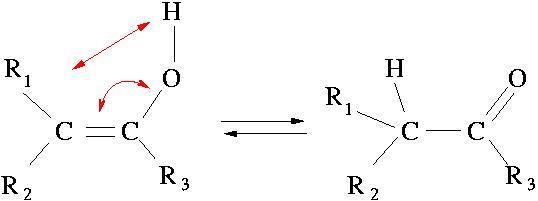
\includegraphics[width=300px]{Figures/s2m/residues/tautomers.png}
  \caption{\label{tautomer}Tautomérie d'une molécule}
\end{figure}

\paragraph{}Les deux transformations présentées ont pour point commun de ne pas modifier en profondeur la structure des molécules.
Dans les deux cas seuls les ``décorateurs'' des labels sont modifiés. Le moyen simple de reconnaître ce type de molécule est alors
d'oublier ces décorateurs lors de la phase d'isomorphisme. Dès lors les résidus sont reconnus quel que soient
leurs variations sur les hydrogènes ou les liens. Cette modification ne fait pas varier la qualité des résultats sur les NRP
car les monomères utilisés différent entre eux au delà des atomes d'hydrogène. Bien que très séduisante cette méthode pose un
problème de temps de calcul.
La plupart des monomères NRP ne contiennent que des composés C N O et H.
Ne pouvant plus utiliser les H comme décorateurs et en rendant les liens indifférents les uns des autres, le nombre de labels différents chute à 9.
Il est donc compréhensible que le temps de calcul augmente beaucoup.

\paragraph{}La solution est une nouvelle fois hybride.
Dans un premier temps, nous cherchons rapidement une solution en effectuant un
isomorphisme contenant tous les labels (isomorphisme {\em strict}), puis en effectuant un pavage et une modulation.
Dans un second temps si aucune solution complète n'est trouvée, nous relançons tout le processus en commençant par
une nouvelle phase d'isomorphisme sans les décorateurs (isomorphisme {\em light}).
Cette seconde phase d'isomorphisme est effectuée localement autour des zones qui ont posé problème lors du premier tour de 
l'algorithme.
Cette algorithme en deux temps nous permet de rapidement traiter tous les cas simples avec des sous algorithmes efficaces puis
de revenir sur les cas plus difficiles avec des algorithmes plus sensibles.

\subsubsection{Vue globale des algorithmes}

\begin{figure}
  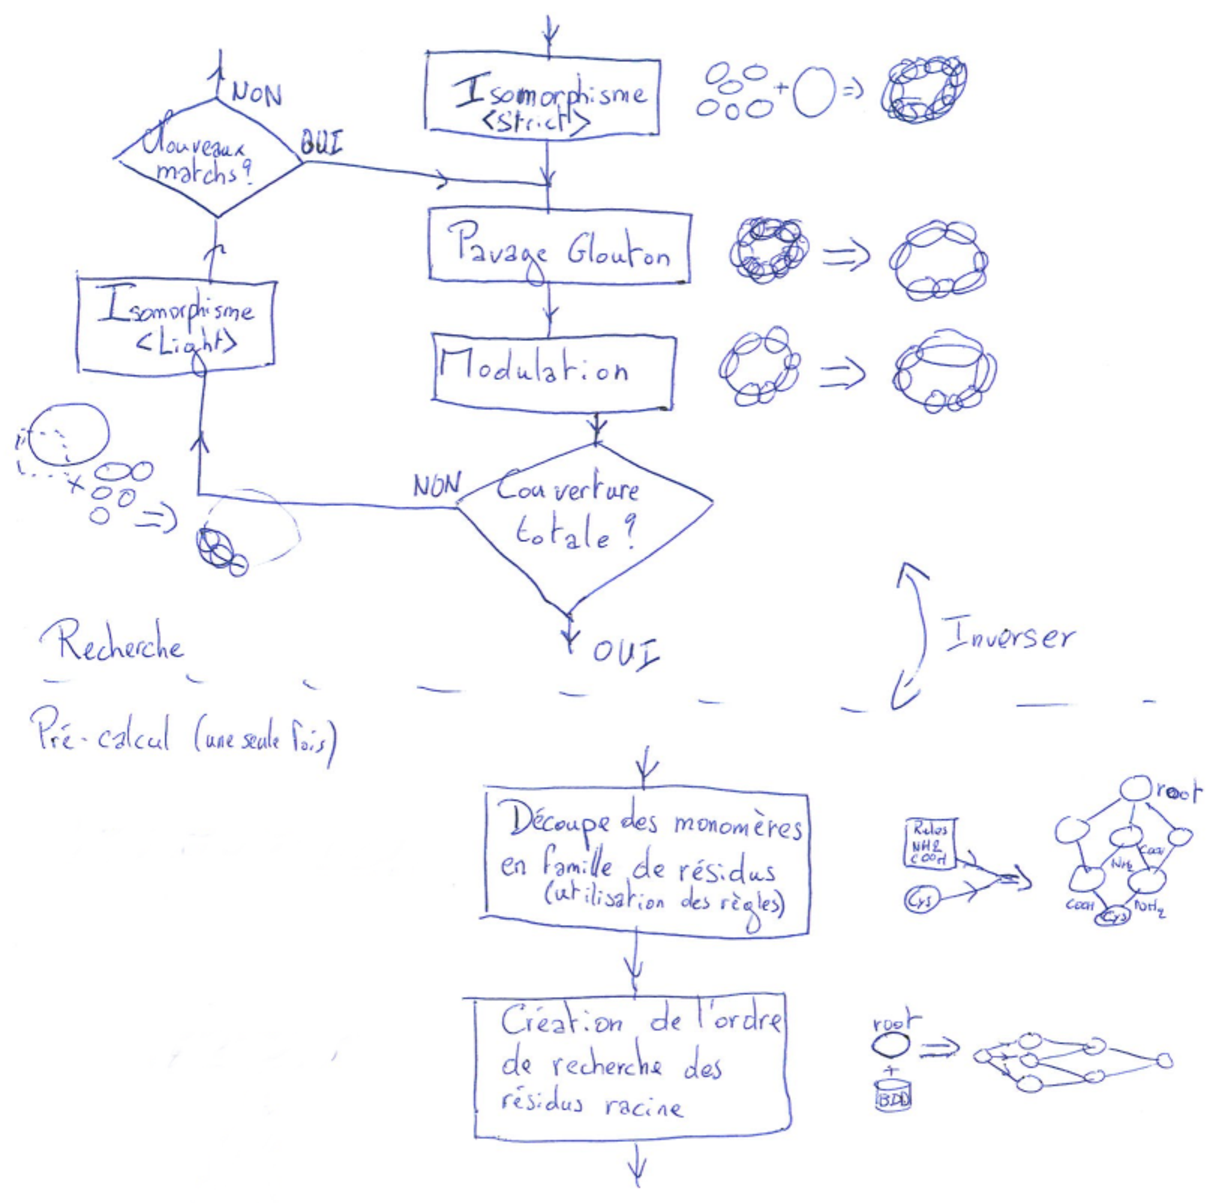
\includegraphics[width=300px]{Figures/s2m/algo/s2m.pdf}
  \caption{\label{global_s2m}Schéma global de Smiles2Monomers}
\end{figure}

\paragraph{}Tout au long cette partie, nous avons présenté par morceaux les différentes parties de Smiles2Monomers.
Nous rassemblons ici tous les morceaux au sein d'un schéma global (figure \ref{global_s2m}).
Le première partie du schéma (au dessus des pointillés) est composée des deux phases de pré-calcul.
Cette étape de pré-calcul est lourde en temps mais n'est à effectuer qu'une seule fois.
Chacune des deux phases de cette étape se déroule en temps exponentiel mais reste calculables grâce à la petite taille des
données.
La seconde moitié du schéma rappelle l'ensemble des étapes comprises dans la phase de recherche. Comme présenté
précédemment, toutes les phases de cette étape sont optimisées afin de minimiser le temps d'exécution de l'algorithme.
La structure en boucle avec l'isomorphisme light nous permet pour la plupart des cas de sortir très vite de l'algorithme.




\subsection{Résultats expérimentaux}

\subsubsection{}





\subsection{Smiles2Monomers en pratique}

\subsubsection{s2m en open source}

\paragraph{}Présentation des méthodes de développement (Github + tests + intégration continue)

\subsubsection{s2m sur NORINE}

\paragraph{}Les utilisations de s2m sur NORINE (Stand alone sur NRP + Correction BDD + 

\subsubsection{Améliorations et limites}

\paragraph{}Discution autour des limites matérielles

\section{Utilisations}











\chapter{Vers la biologie de synthèse}

\bibliography{these}
\bibliographystyle{plain}

\end{document}          
